\chapter{Design Trade-Off}
\label{ch:trade-off}
In this Chapter, the preliminary HUGO configurations developed in previous design stages are compared by means of a trade-off. Suitable trade-off criteria are defined in \autoref{sec:trade-off_criteria_selection}, followed by a definition of weight factors in \autoref{sec:trade-off_weight_factors}. The results of the trade-off analysis are presented in \autoref{sec:trade-off_matrix}, and the final configuration to be further developed can be found in \autoref{sec:trade-off_final_design}. Additionally, a material selection trade-off is performed in \autoref{sec:Material_Selection}. 

\autoref{tab:Final_Candidate_Architectures} lists the design configurations considered for the trade-off. Additionally, each design option features a static port for the tail, fuselage-mounted fuel tanks and fuselage-mounted engines \footref{url:baseline_report}.

\begin{table}[H]
    \centering
    \caption{Final Integrated Candidate Architectures for Detailed Trade-Off \footref{url:baseline_report}}
    \label{tab:Final_Candidate_Architectures}
    \renewcommand{\arraystretch}{1.3}
    %\resizebox{\textwidth}{!}{% Scales table to fit the page width if it gets too wide
    \begin{tabular}{|c|c|c|c|c|}
        \hline
        \textbf{ID} & \textbf{Wing Configuration} & \textbf{Wing Modularity} & \textbf{Canard Modularity} & \textbf{Gear Type}    \\
        \hline\hline
        HUG-CFG-301 & Low Wing & Variable Port (X) & Static Port & Retractable Buried \\
        \hline
        HUG-CFG-302 & High Wing & Static Port & No Port & Side Podded \\
        \hline
        HUG-CFG-303 & High Wing & Static Port & Static Port & Retractable Buried \\
        \hline
        HUG-CFG-304 & High Wing & Variable Port (X) & Static Port & Side Podded \\
        \hline
        HUG-CFG-305 & High Wing & Variable Port (X) & Static Port & Retractable Buried \\
        \hline
    \end{tabular}
\end{table}

As the changes between considered configurations lay mostly in the modularity details and landing gear types, a separate trade-off will be performed concurrently to determine the most suitable materials for different subsystems of the final configuration. Candidate will be discussed in \autoref{sec:Material_Selection}.

\begin{figure}[H]
    \centering

    \begin{subfigure}[t]{0.48\textwidth}
        \centering
        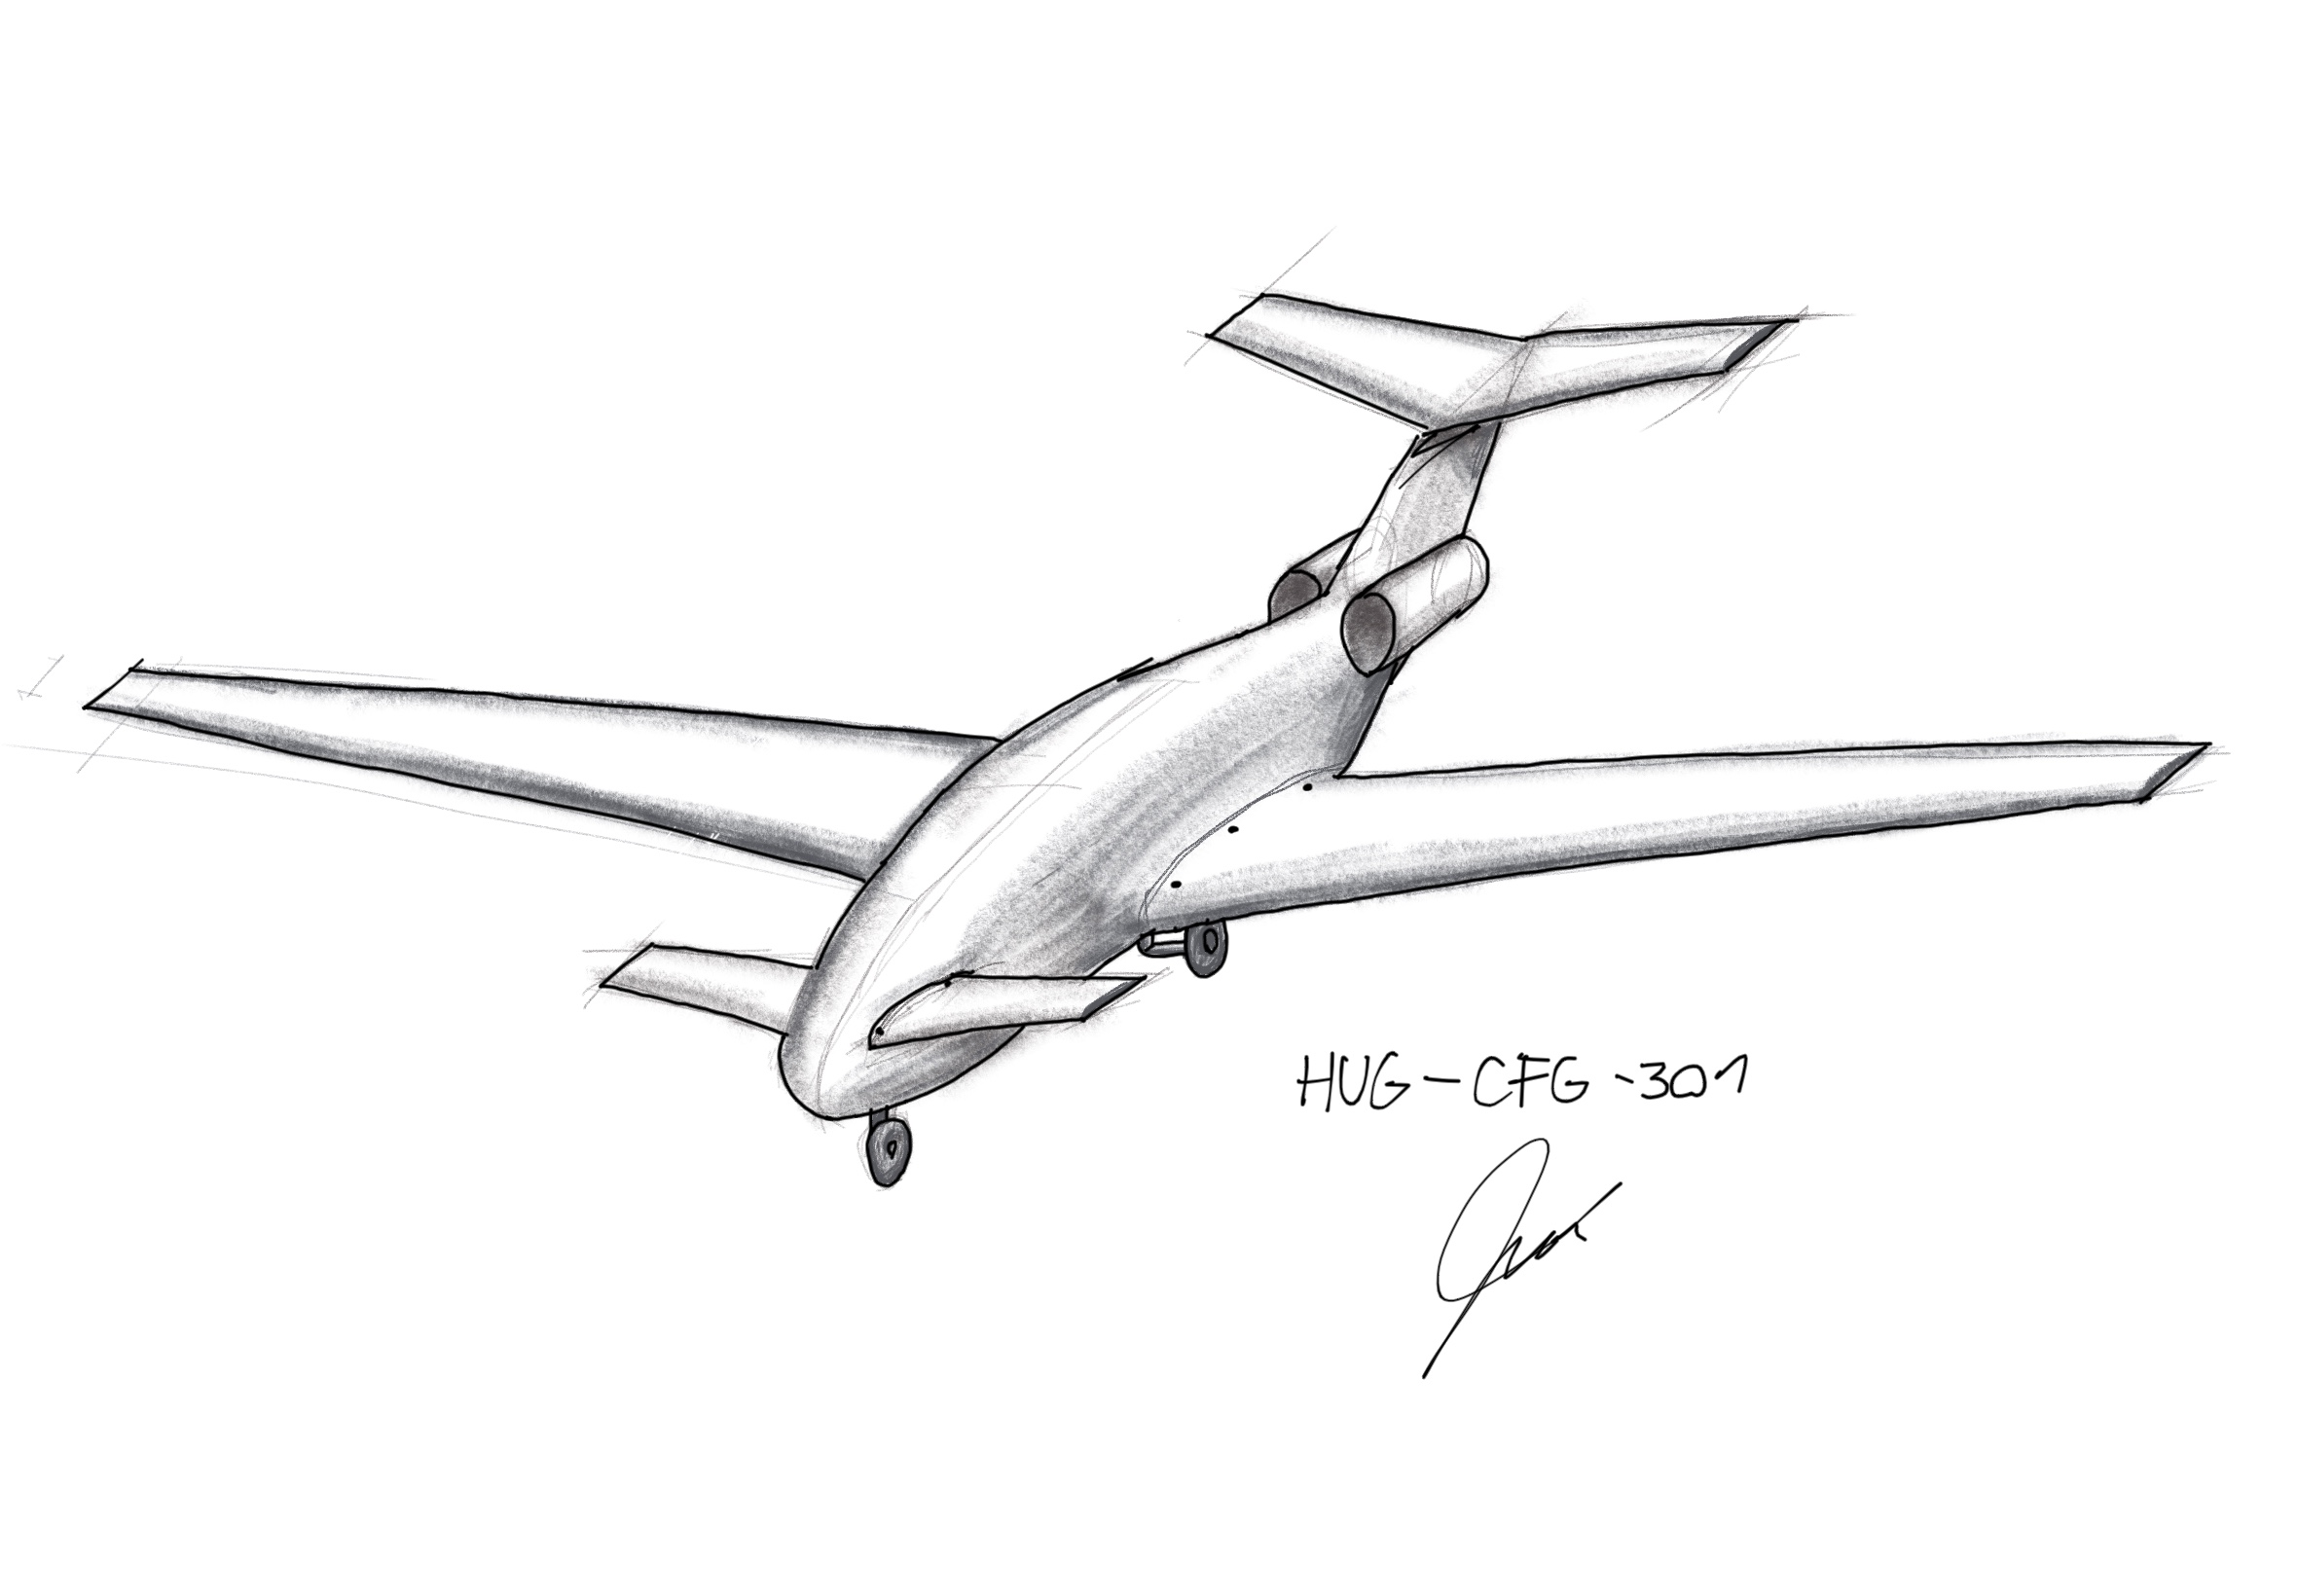
\includegraphics[width=\linewidth]{figures/Sketches/HUG-CFG-301.jpeg}
        \caption{HUG-CFG-301: low wing, static wing port, no canard port, buried retractable landing gear}
        \label{fig:hug-cfg-301}
    \end{subfigure}
    \hfill
    \begin{subfigure}[t]{0.48\textwidth}
        \centering
        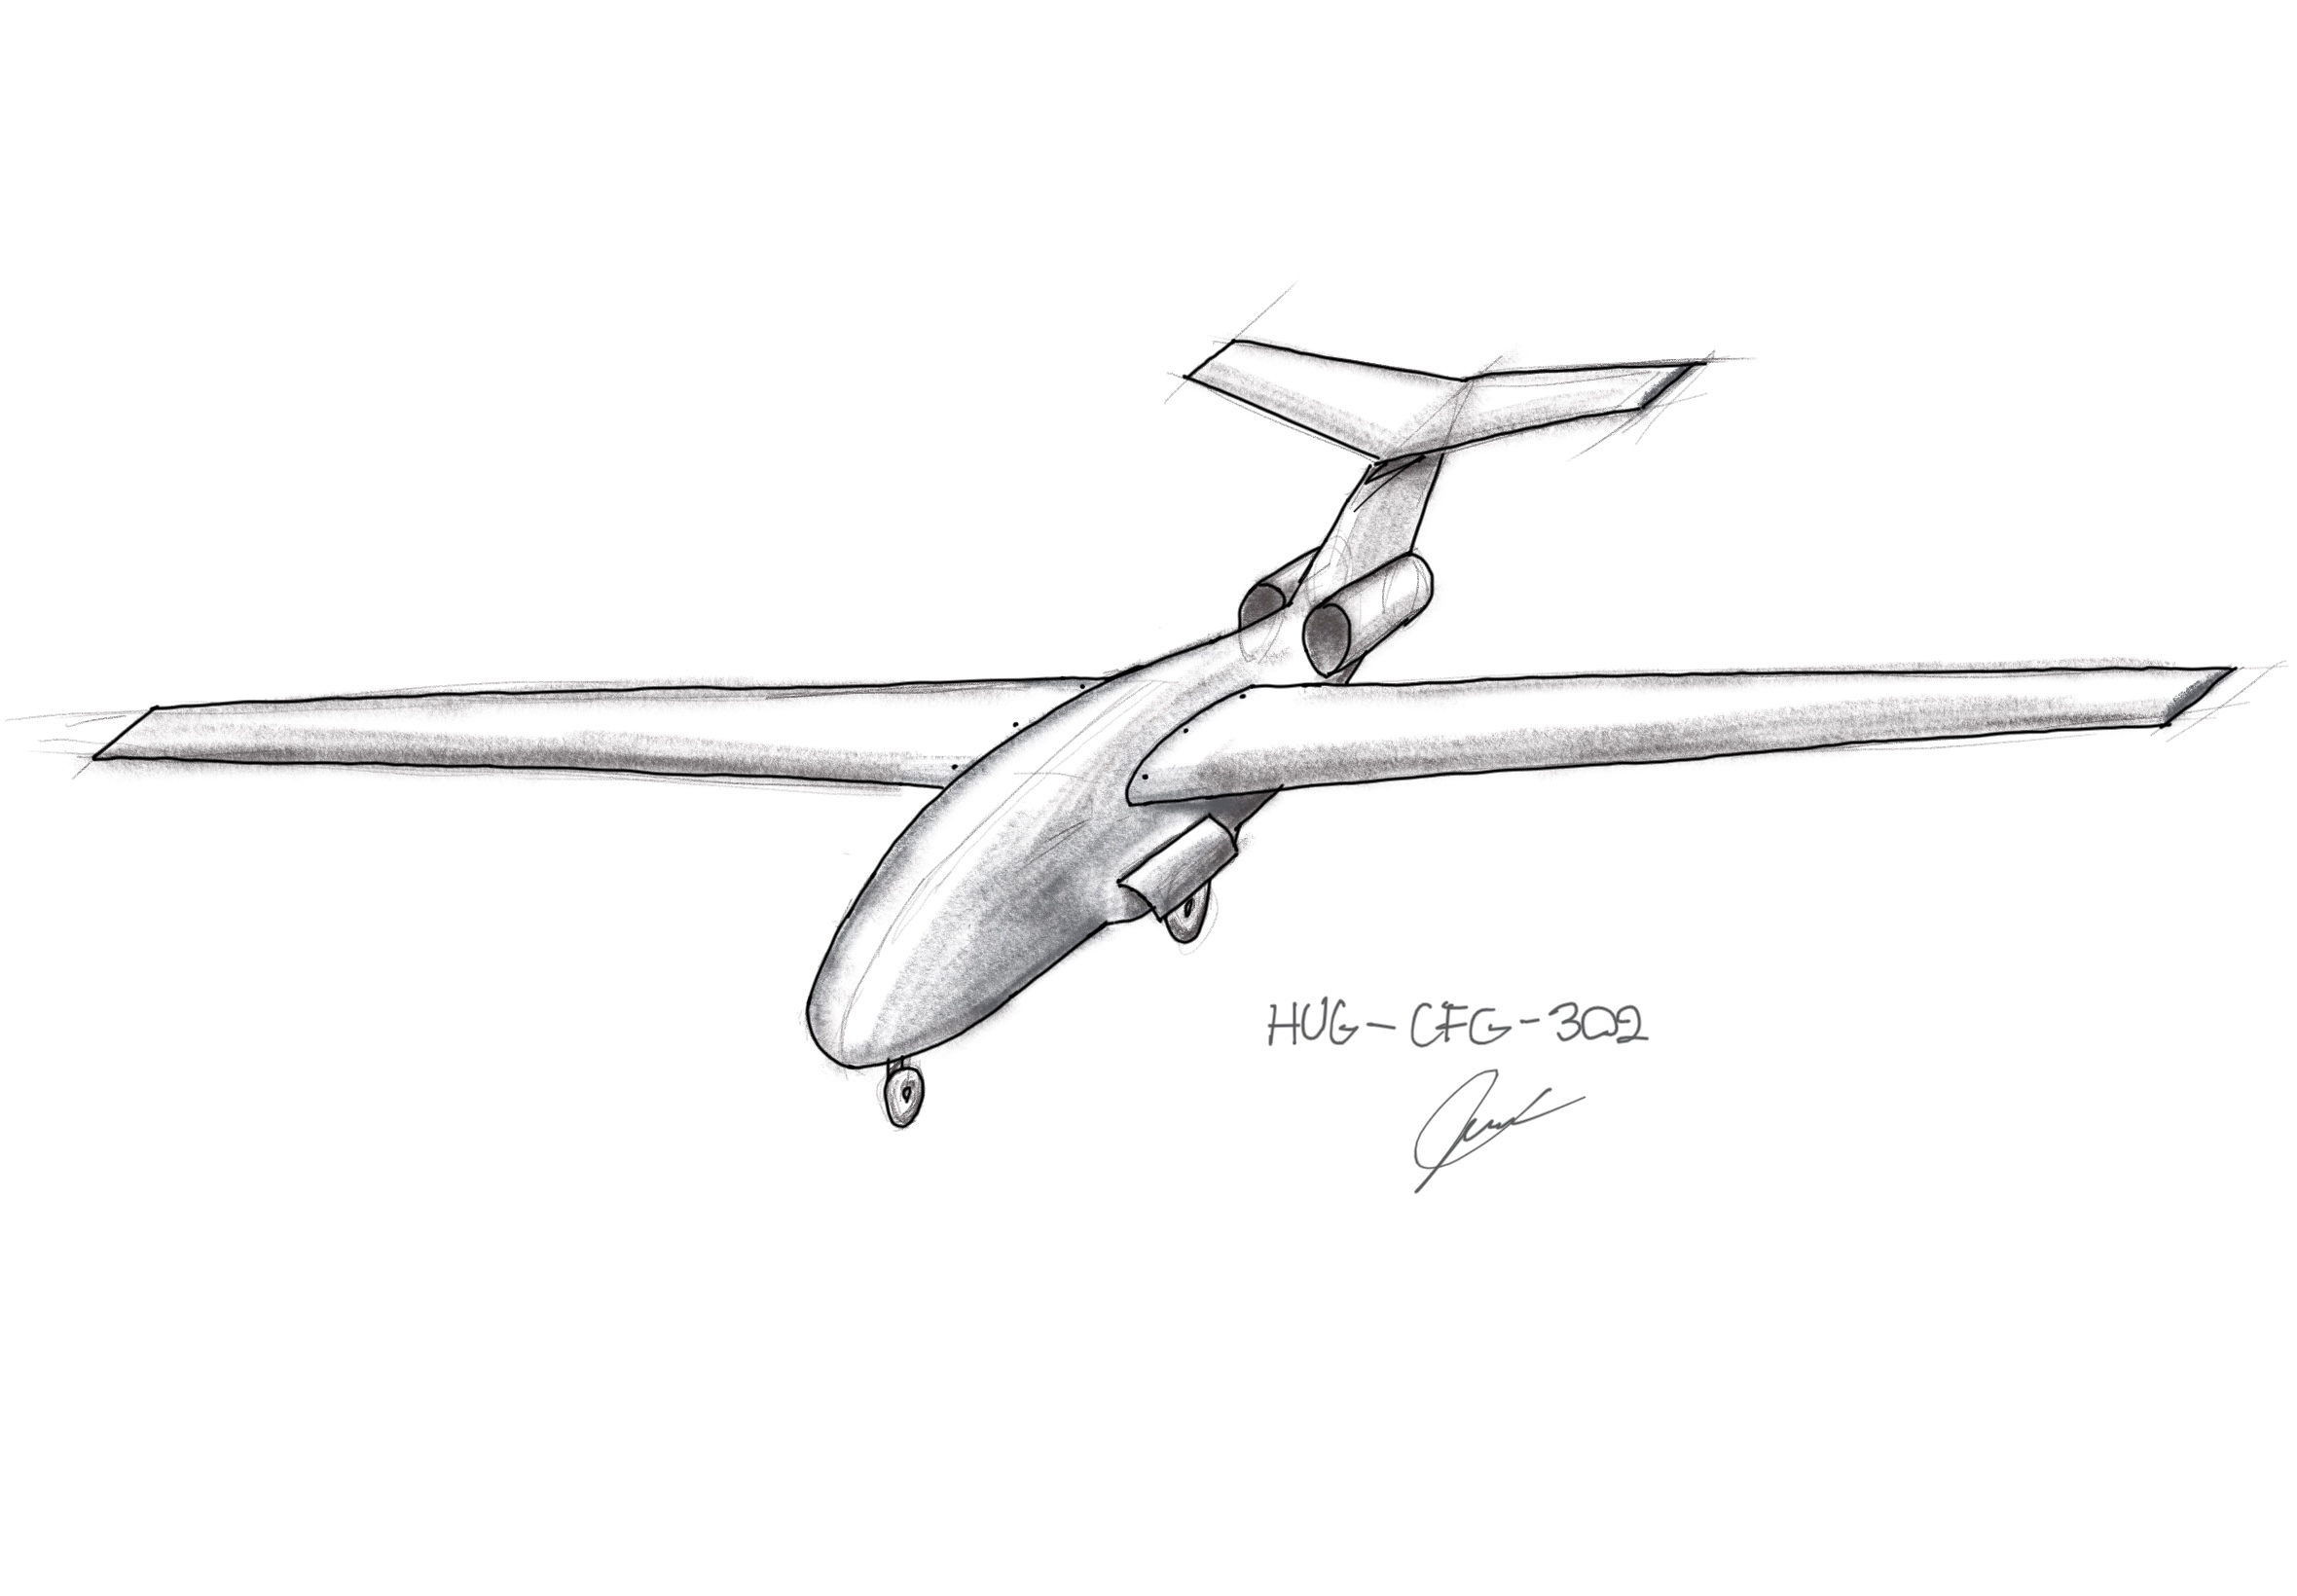
\includegraphics[width=\linewidth]{figures/Sketches/HUG-CFG-302.jpeg}
        \caption{HUG-CFG-302: low wing, variable wing port, no canard port, side-podded retractable landing gear}
        \label{fig:hug-cfg-302}
    \end{subfigure}

    \caption{Initial HUGO configuration concepts}
    \label{fig:hugo-configurations-301-302}
\end{figure}


\begin{figure}[H]
    \centering

    \begin{subfigure}[t]{0.48\textwidth}
        \centering
        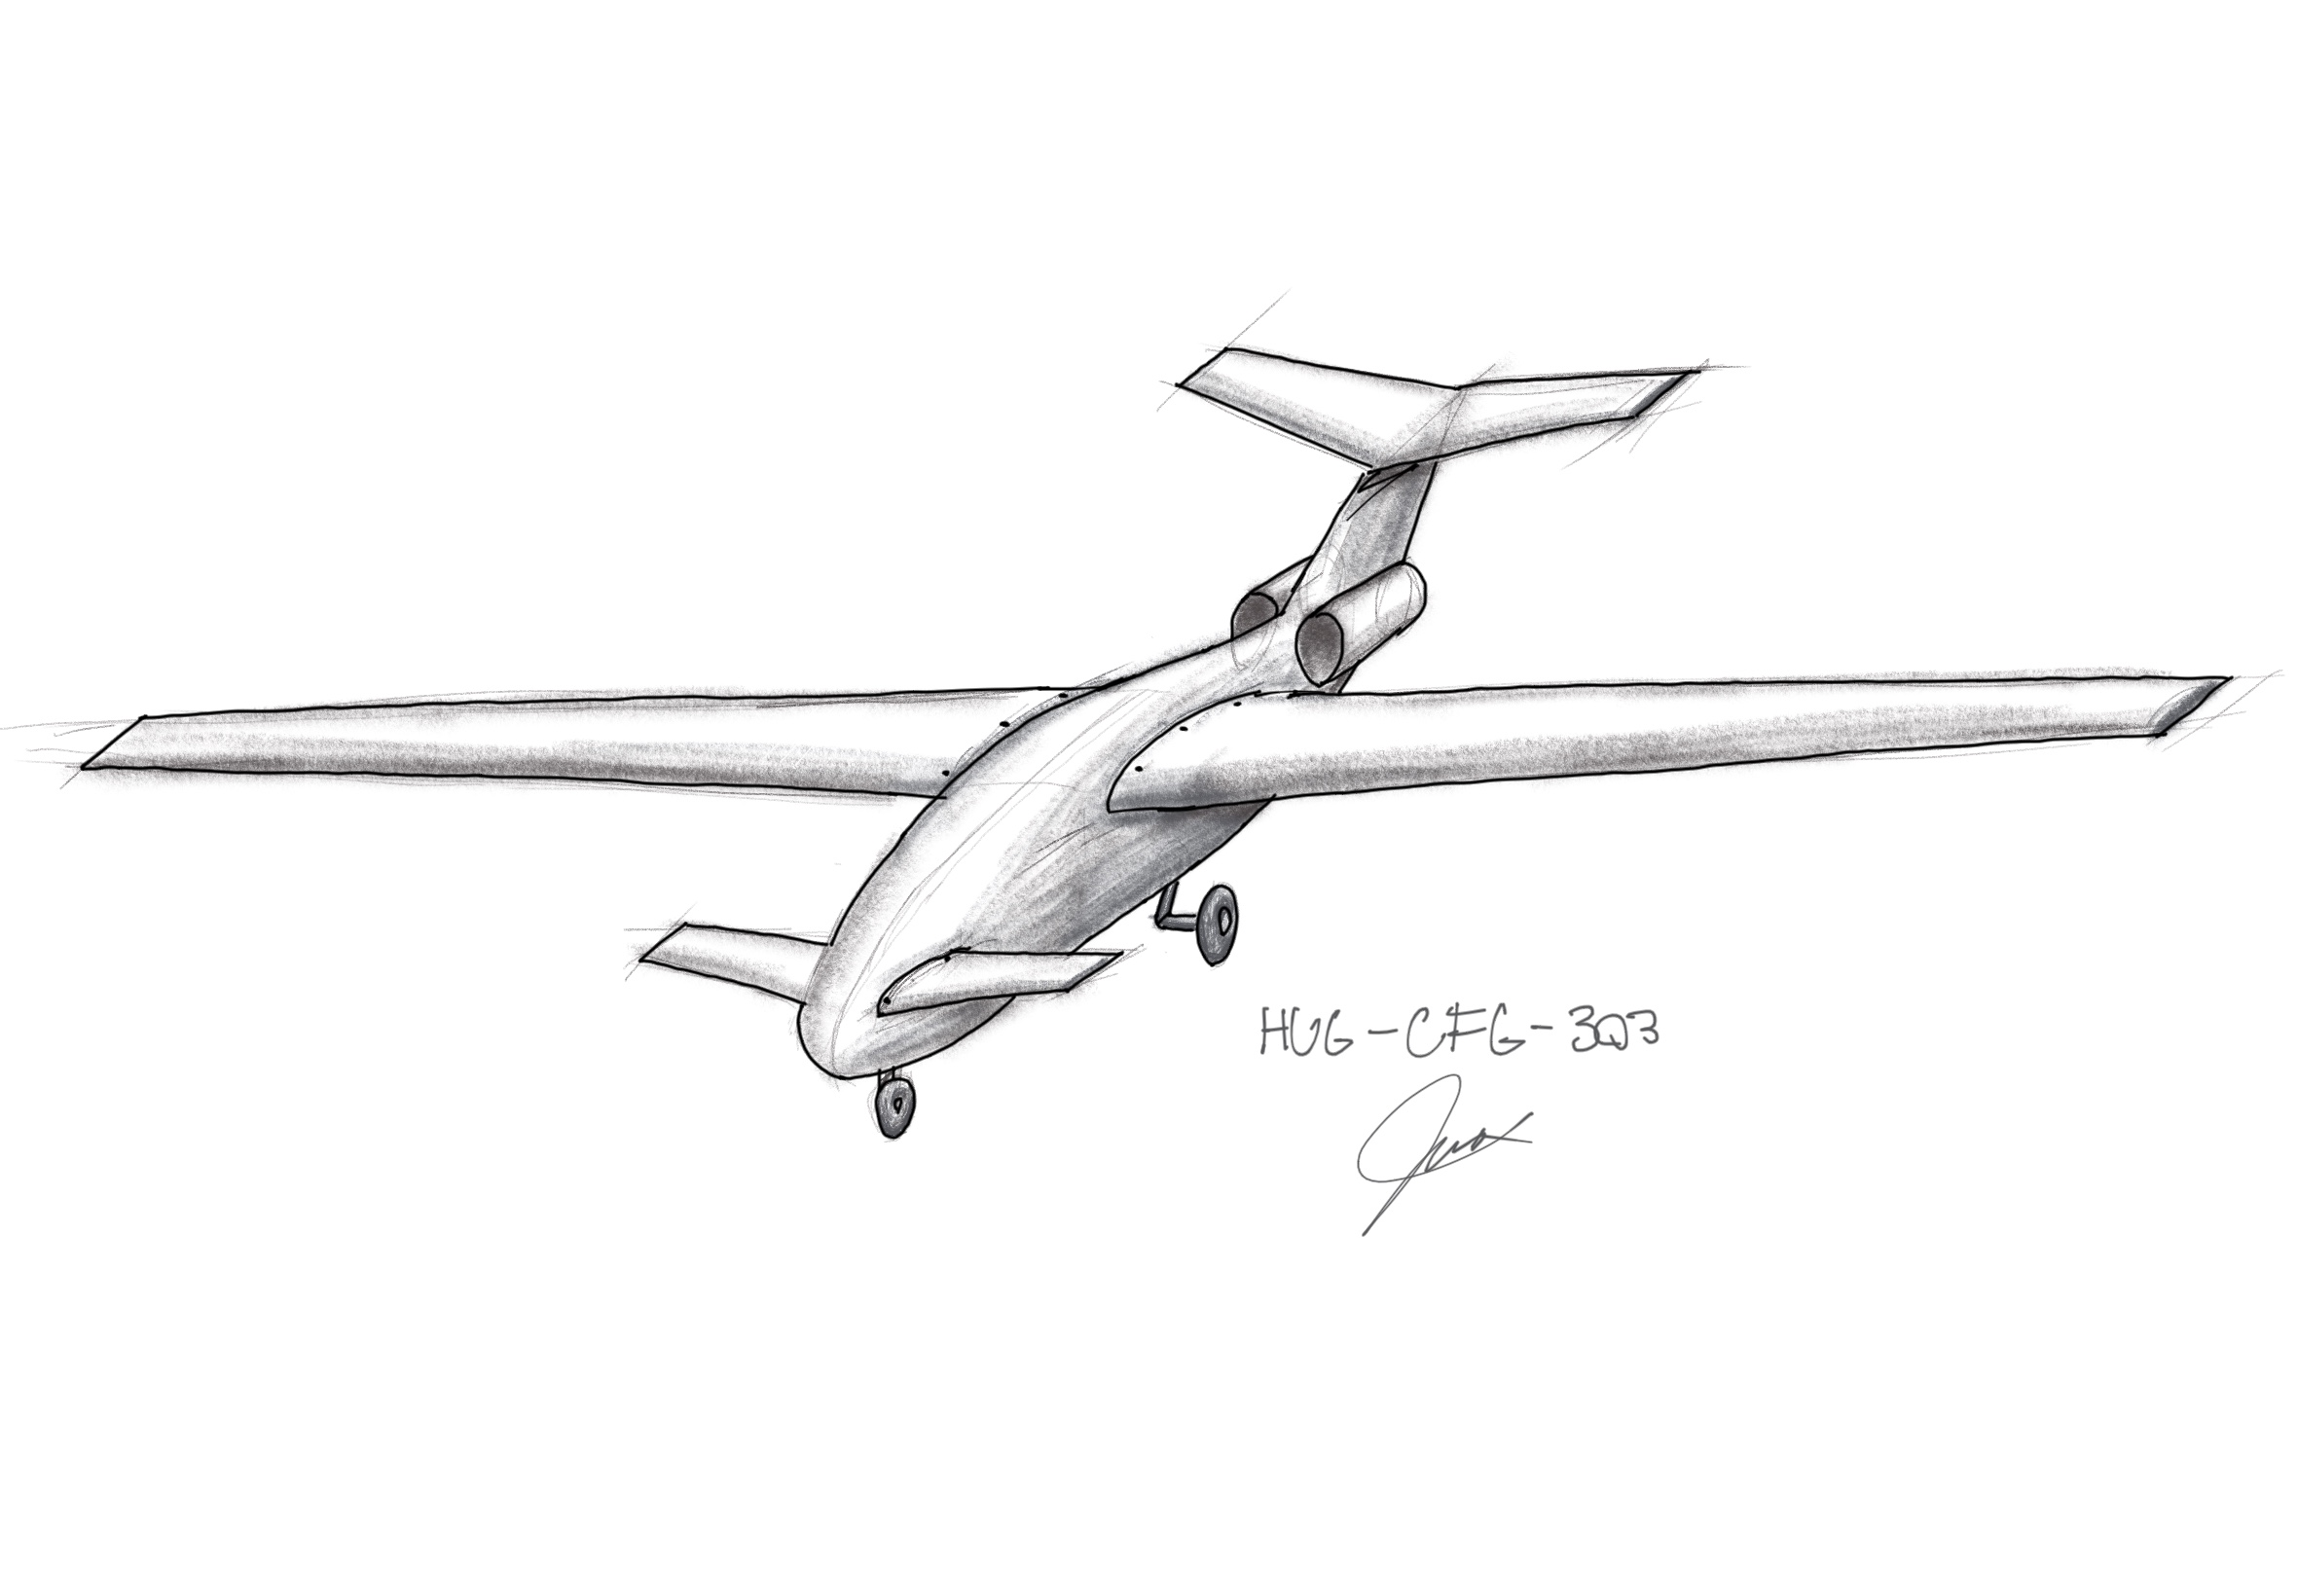
\includegraphics[width=\linewidth]{figures/Sketches/HUG-CFG-303.jpeg}
        \caption{HUG-CFG-303: high wing, static wing port, static canard port, buried retractable landing gear}
        \label{fig:hug-cfg-303}
    \end{subfigure}
    \hfill
    \begin{subfigure}[t]{0.48\textwidth}
        \centering
        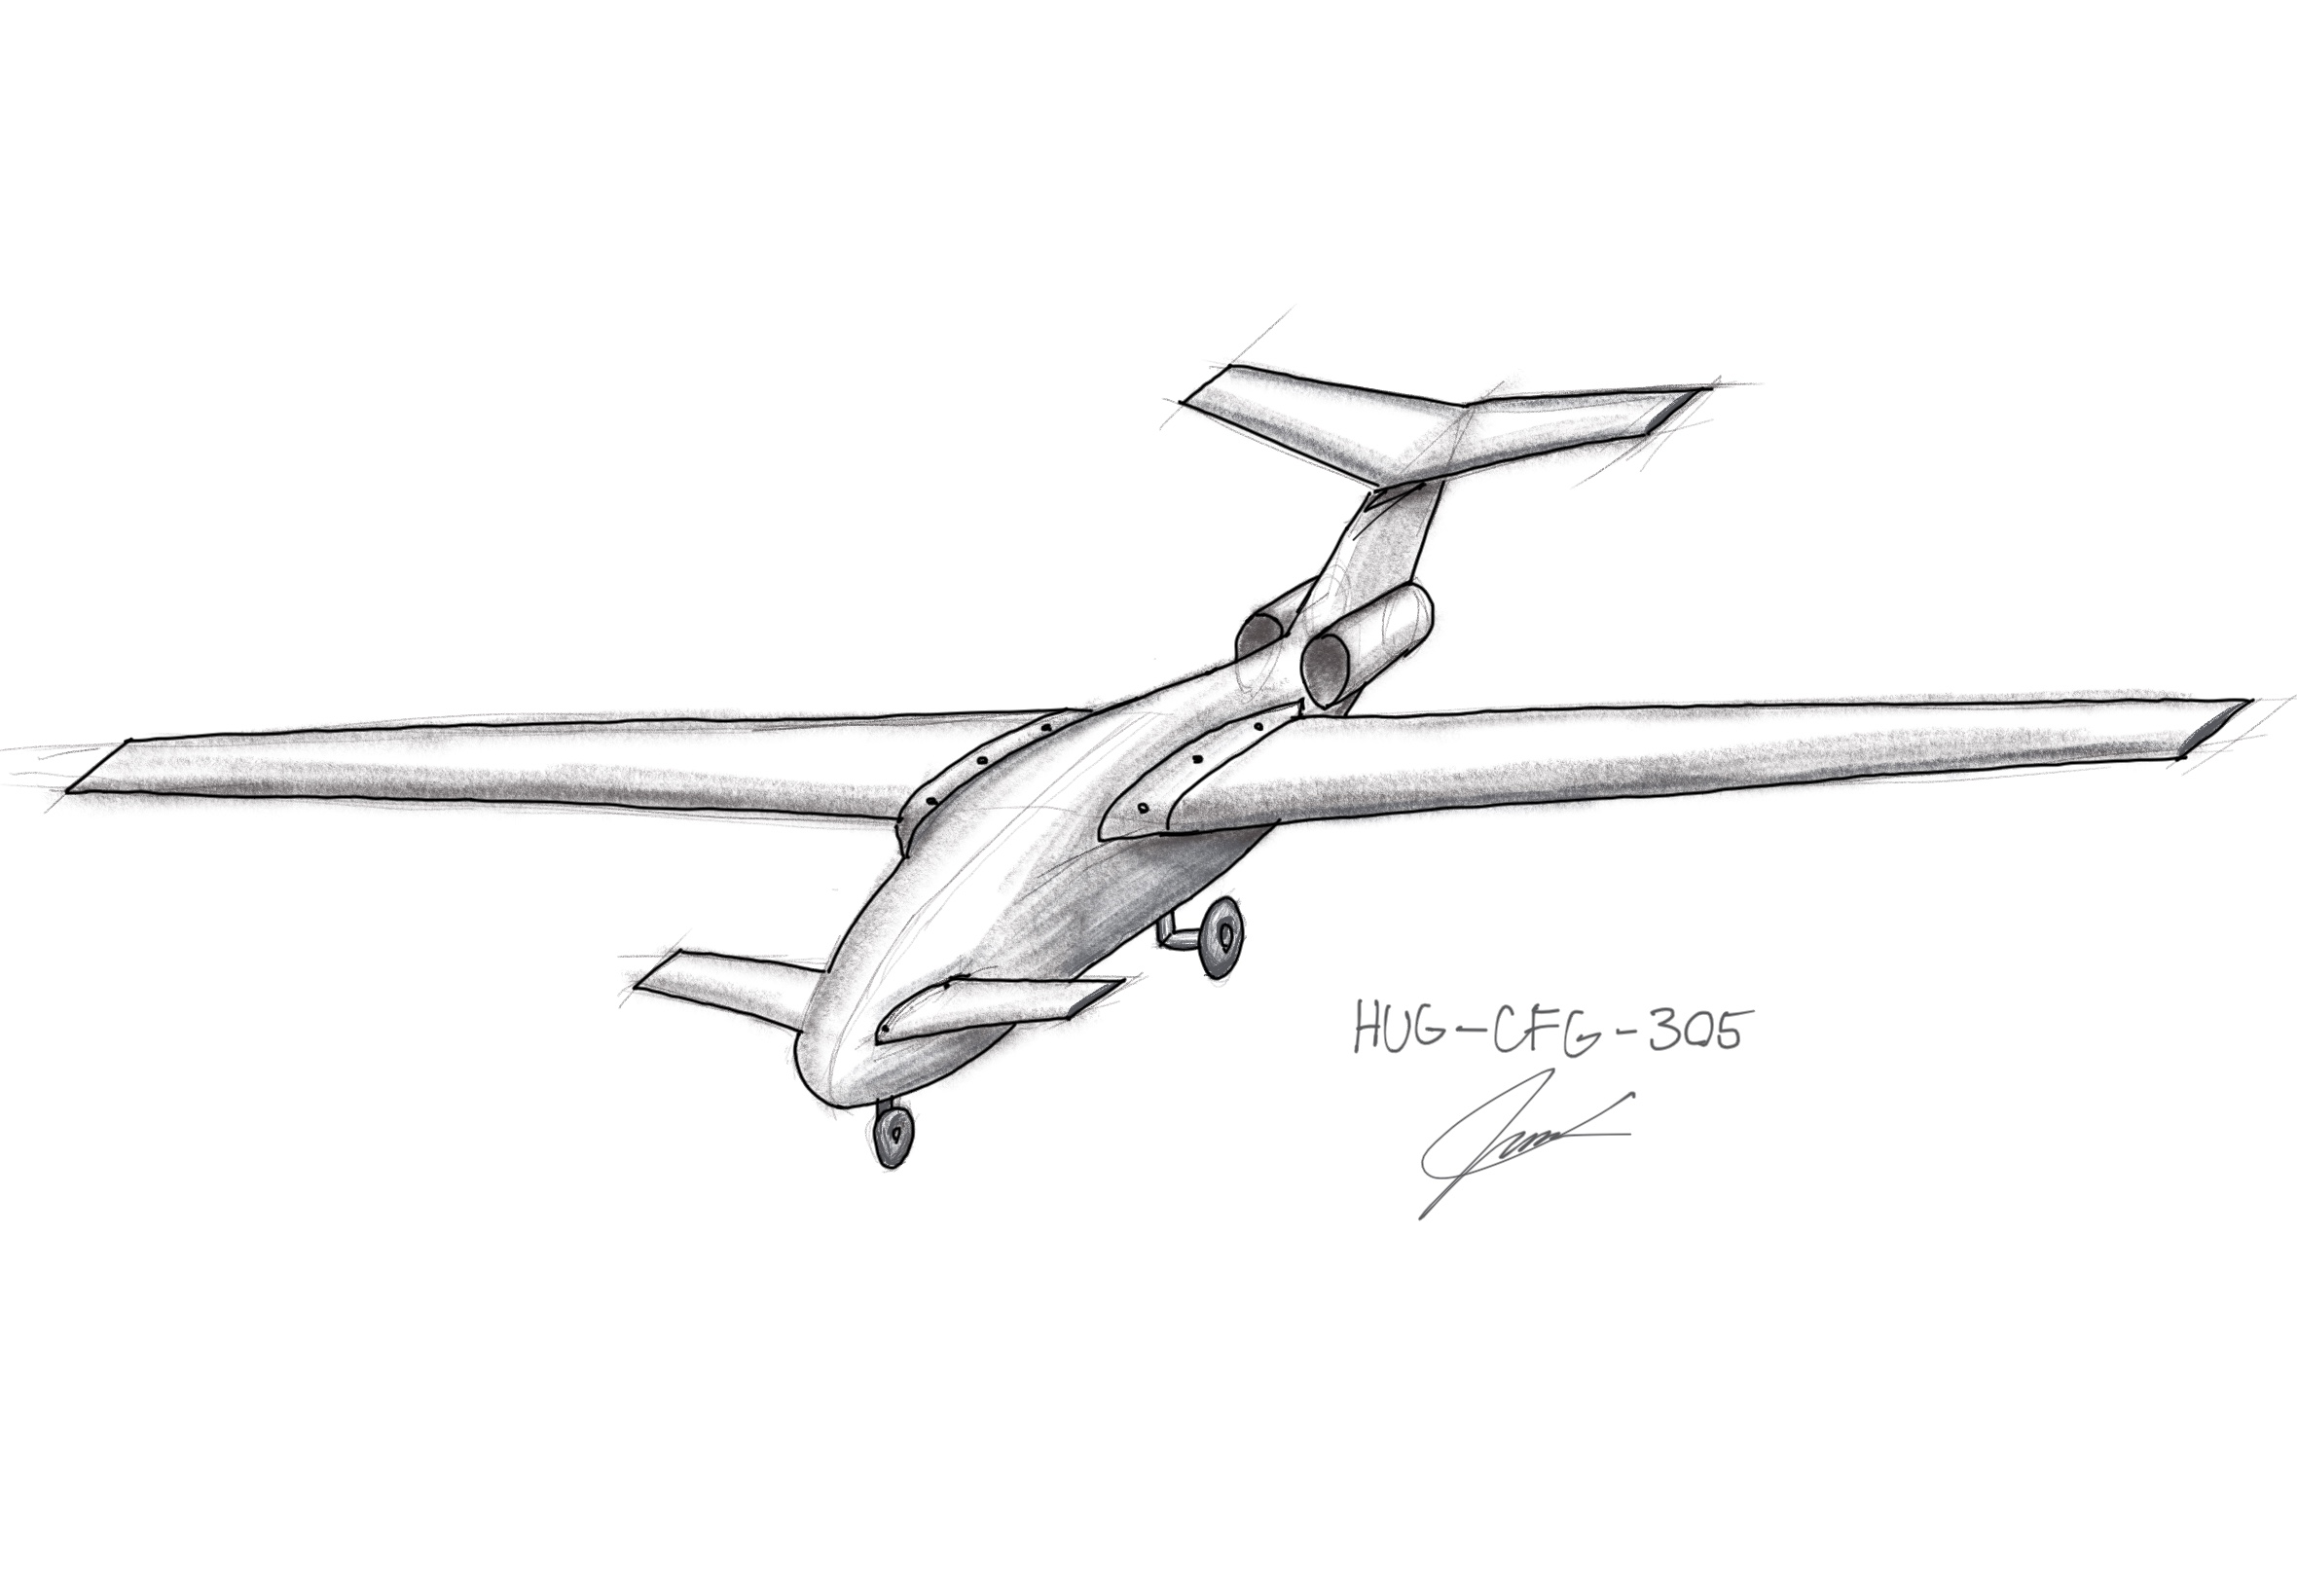
\includegraphics[width=\linewidth]{figures/Sketches/HUG-CFG-305.jpeg}
        \caption{HUG-CFG-305: high wing, variable wing port, static canard port, buried retractable landing gear}
        \label{fig:hug-cfg-305}
    \end{subfigure}

    \caption{Initial HUGO configuration concepts}
    \label{fig:hugo-configurations-303-305}
\end{figure}

\begin{figure}[H]
    \centering

    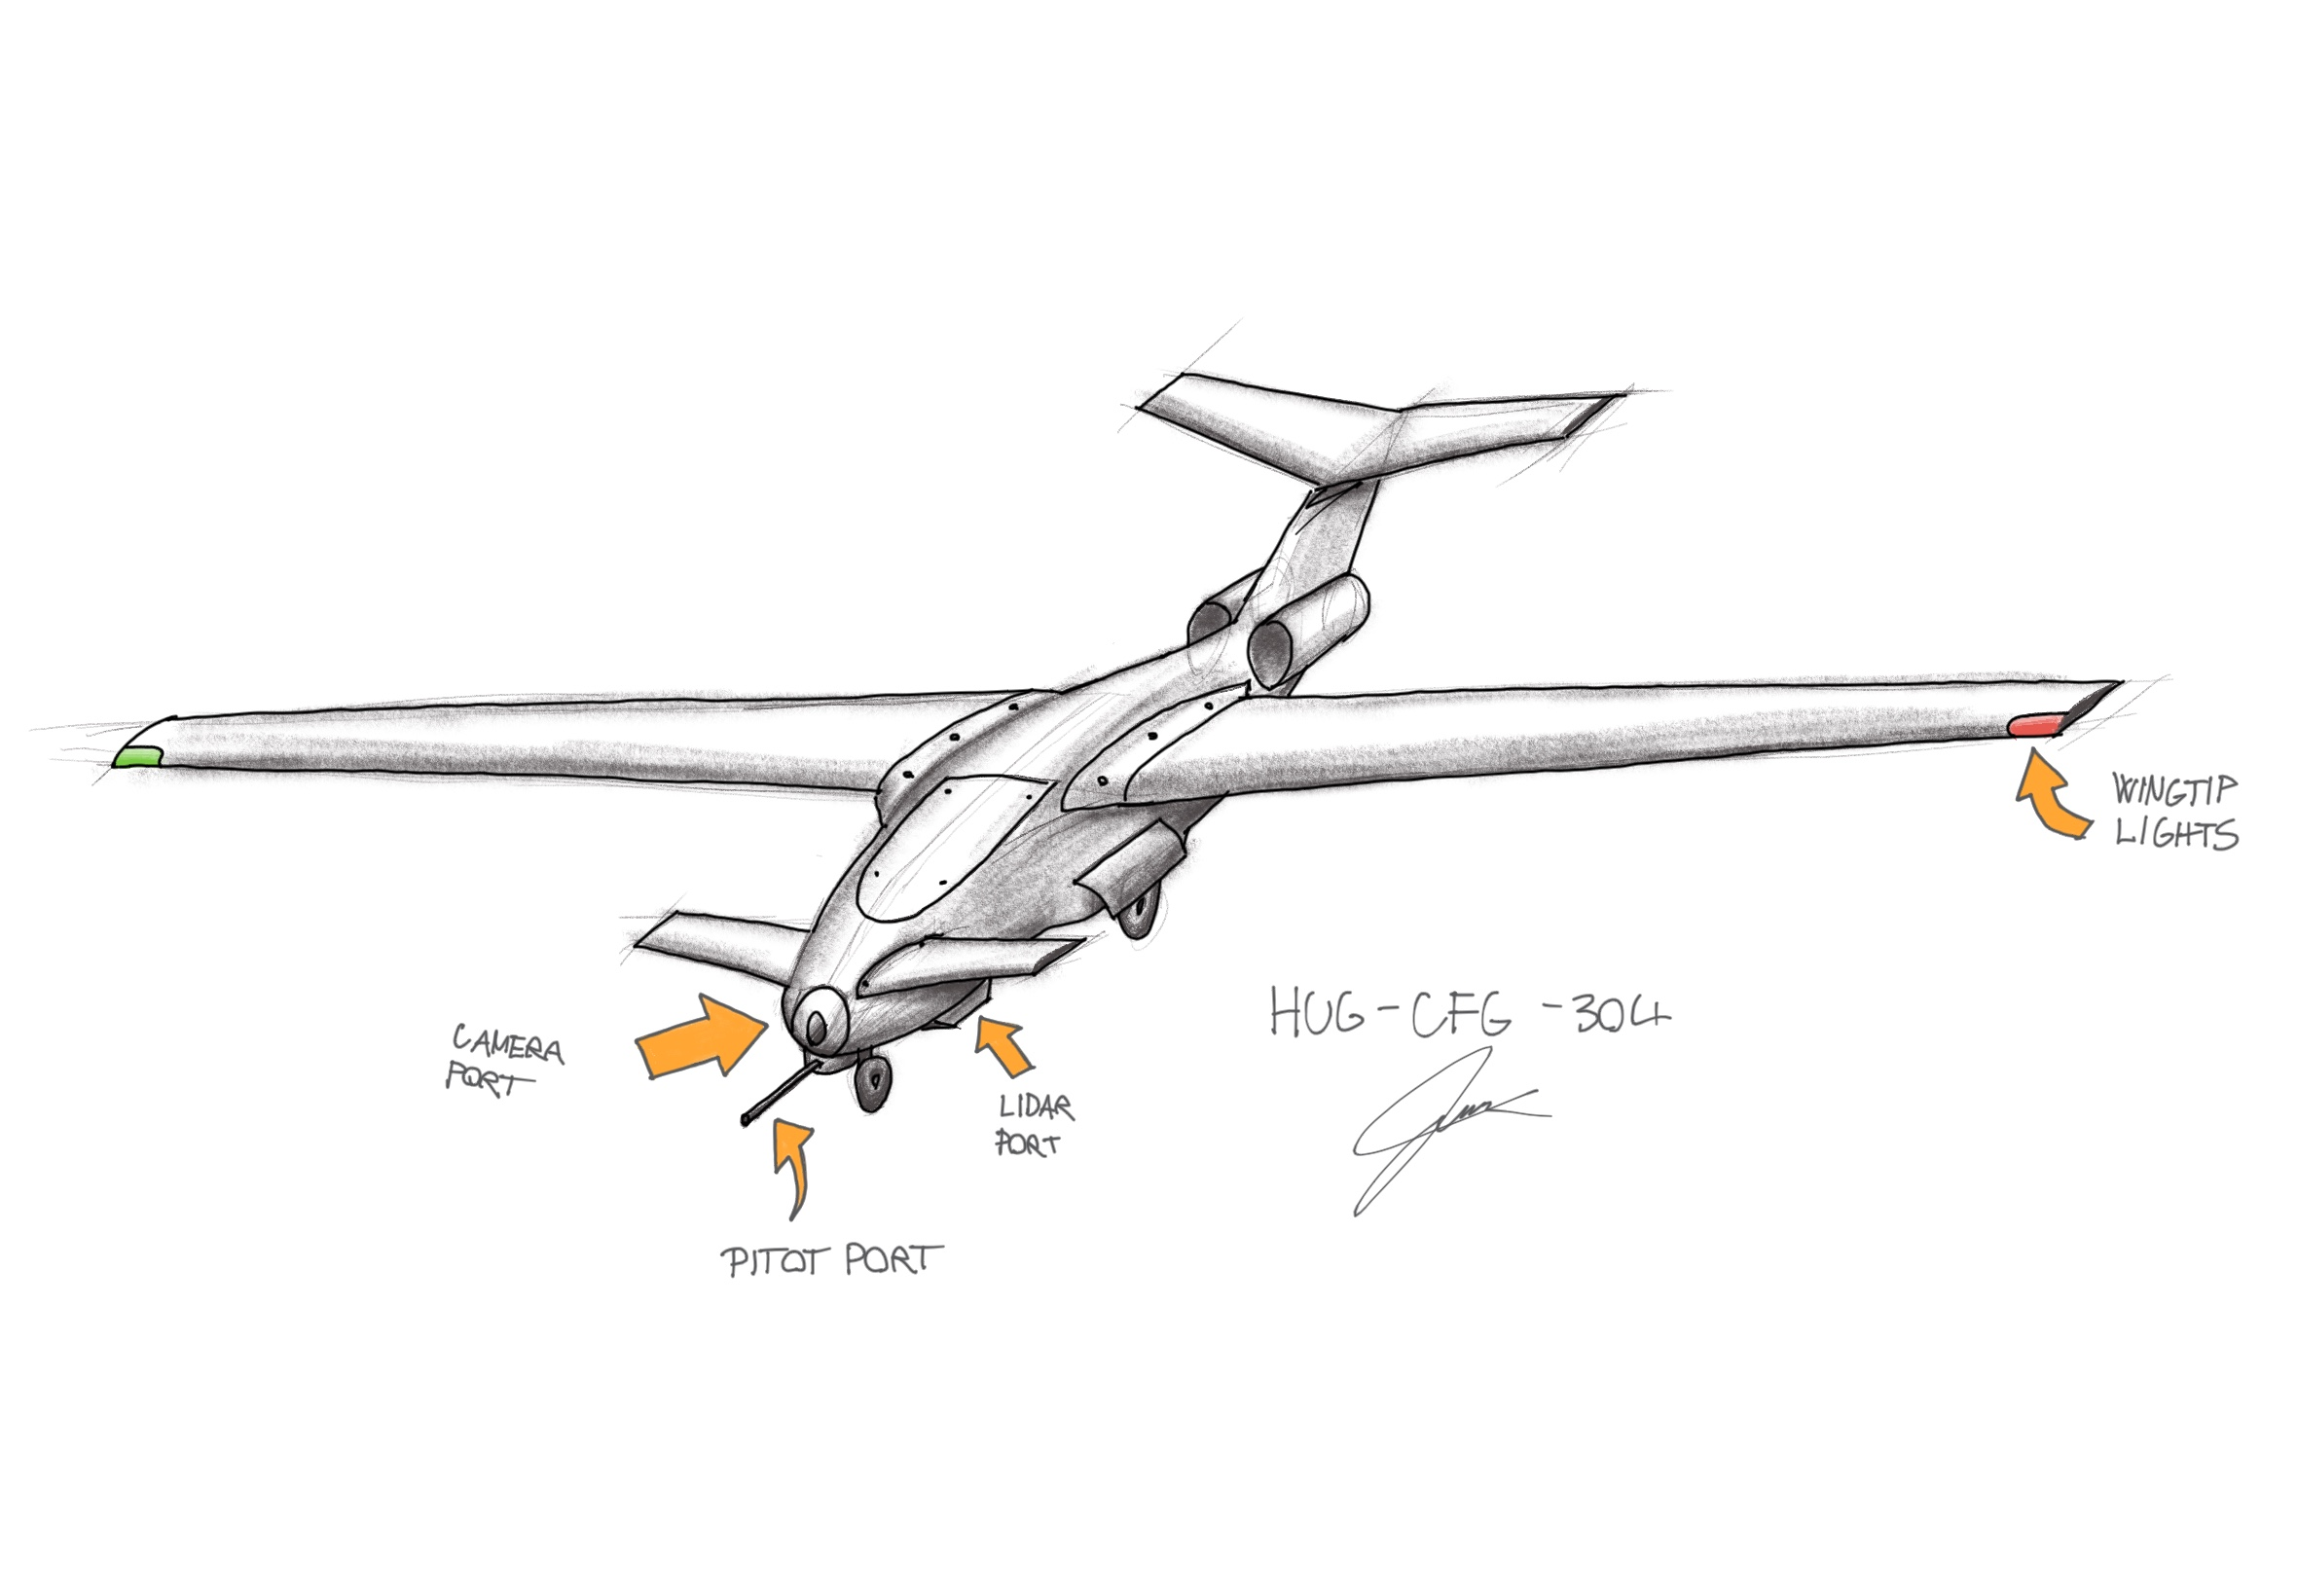
\includegraphics[width=\textwidth]{figures/Sketches/Outer_Stuff.jpeg}

    \caption{HUG-CFG-304: high wing, variable wing port, static canard port, side-podded retractable landing gear; with an example external instrument layout}
    \label{fig:hug-cfg-304-outer}
\end{figure}

\section{Trade-Off Criteria Selection}
\label{sec:trade-off_criteria_selection}
Meaningful trade-off criteria should be developed such that all available technical specifications and key performance metrics are considered. Moreover, identifying the points of poor performance of each candidate allows for an in-depth analysis of the limitations of each candidate configuration \cite{SMAD}. Lastly, the key requirements can be used to ensure that the developed criteria encompass all crucial design aspects.
%It is not helpful to include criteria where all options perform similarly; instead, it is more valuable to use criteria where some options perform poorly, as this helps reveal and compare weaknesses across designs. In this way, each design’s limitations can be properly assessed. In addition, some of the requirements identified in the baseline review can also serve as a basis for defining the trade-off criteria.

Taking all of the above into consideration, the following criteria were selected for the trade-off of HUGO designs: Versatility, Reliability, Cost, Performance, and Sustainability. \autoref{tab:trade-off_criteria} lists the rationale behind selecting each criterion for the configuration trade-off, while \autoref{sec:Mat_sel} lists those used for the material trade-off.

\begin{longtable}{|p{2.5cm}|p{13.5cm}|}
\caption{Trade-Off Criteria for HUGO Configurations}
\label{tab:trade-off_criteria} \\

\hline
\textbf{Criterion} & \textbf{Rationale} \\ 
\hline
\endfirsthead

\hline
\textbf{Criterion} & \textbf{Rationale} \\ 
\hline
\endhead

\hline
\multicolumn{2}{r}{\textit{Continued on next page.}} \\
\endfoot

\hline
\endlastfoot

Versatility & HUG-CFG-301 is a low wing concept that prevents the testing of truss-braced wing concepts, which was considered significant in conversations with NLR. Similarly, HUG-CFG-302 prevents the testing of canard-dependent configurations, which limits the range of possible test scenarios, including the testing of canard configurations and mounting scaled wing models in front of the main planform.\\ \hline

Reliability & Variable wing ports in HUG-CFG-301, HUG-CFG-304, and HUG-CFG-305 introduce additional fatigue exposure at modular interfaces, increasing operational risk. Buried retractable gear in HUG-CFG-301, HUG-CFG-303, and HUG-CFG-305 reduces accessibility for maintenance of the retraction mechanism. Moreover, the design of HUGO is subject to specific reliability requirements (see: HUG-STR-003 \footref{url:baseline_report}).\\ \hline

Cost & Variable wing ports featured in HUG-CFG-301, HUG-CFG-304, and HUG-CFG-05 significantly increase the design complexity and associated development, maintenance and repair costs compared to no/static port configurations. The same reasoning can be applied to retractable landing gear mechanisms for HUG-CFG-302, HUG-CFG-304 due to the additonal podded complexity. Moreover, the design of HUGO is subject to specific cost requirements (see: HUG-FIN-001 \footref{url:baseline_report}). \\ \hline

Performance & Complex design options featured in HUG-CFG-301, HUG-CFG-304, and HUG-CFG-305 are expected to result in higher design weights, which affect performance and fuel consumption. Moreover, the design of HUGO is subject to specific performance requirements (see: HUG-OPS-005, HUG-OPS-006 \footref{url:baseline_report}). The type of landing gear was also part of the grading process, as it was analysed in \autoref{sec:Landing_gear_config}, HUG-CFG-302 and HUG-CFG-304 scoring lower due to the podded added drag.
\\ \hline

Sustainability & Sustainability is part of the project, as specified by HUG-OPS-008 \footref{url:baseline_report}. Variable ports and podded retractable undercarriage require more material, more complex manufacturing processes, more labour hours in assembly and quality control, and higher maintenance material consumption over the aircraft's life.
\\

\end{longtable}


\begin{comment}
\begin{enumerate}
    \item Versatility was selected since configuration 2 prevents the testing of canard-dependent configurations, and the variable ports in configurations 1, 4, and 5 allow for a wider range of stability conditions to be tested. This means that some of the options will score low in this criterion. 
    \item Reliability was considered a crucial trade-off criterion since the variable port in configurations 1, 4, and 5 significantly increases the risk of failure, and also the development risk. Additionally, ports and gear bays weaken the primary structure of the aircraft. This was also derived from requirement HUG-STR-003 \cite{Baseline report}, specifying the required reliability of the structure. 
    \item Considering also that variable ports and retractable landing gear are significantly more complex and expensive in comparison to no/static port and buried gear, cost was selected as another trade-off criterion. 
    \item The performance criterion stems from several requirements from the baseline report specifying the required speed (HUG-OPS-005, HUG-OPS-006 \cite{Baseline report}), and also the insight that more complex configurations like 1, 4, and 5 will lead to a higher mass, and thus affect the performance and fuel burn.
    \item Sustainability is part of the project, as specified by HUG-OPS-008 \cite{Baseline report}. Additionally, variable ports and retractable undercarriage require more material, more complex manufacturing processes, more labour hours in assembly and quality control, and higher maintenance material consumption over the aircraft's life.
\end{enumerate}
\end{comment}

The preliminary configurations and materials shall be evaluated and assigned a value ranging from 1 to 5 in each trade-off criterion. The definition of specific scores for different criteria can be found in \autoref{ch:app_trade-off_rationale}. The following rationale was followed in quantifying the scores for individual criteria for the configurations:
\begin{itemize}
    \item \textbf{Versatility} is quantified as the range of experiments and stability conditions that can be tested with the given configuration. As mentioned above, a configuration that can not test canard configurations or has a static port will score lower.
    \item \textbf{Performance }is evaluated based on how effectively the maximum Mach number at test altitude can be achieved while carrying the full instrumentation payload, with minimal drag and fuel consumption. Configurations that are lighter, less complex, and feature fewer protruding components will receive higher scores.
    \item \textbf{Reliability} is evaluated as the likelihood that the testbed successfully performs its intended function without failure under specified operating conditions throughout its lifetime. Mainframe fatigue at modular interfaces and maintenance accessibility are identified as primary reliability drivers. Accessibility determines the feasibility of preventive maintenance, directly affecting whether soft failures can be detected and corrected before escalating. Scores reflect the severity of anticipated failure modes, from soft failures causing minor performance degradation to severe failures risking significant structural damage.
    \item \textbf{Cost} is quantified as the manufacturing effort, materials, development, and maintenance that have gone into each configuration. More complex and heavier designs will score lower here.
    \item \textbf{Sustainability} is quantified as the manufacturing complexity and material consumption, penalised by number of moving parts, material types, and estimated labour hours. Configurations with more moving parts, additional material types, and higher labour requirements score lower.
\end{itemize}

%The no-go values (ranging from 1 to 5) of the criteria were also estimated. They are given in \autoref{tab: no-go} with a short rationale. A more in-depth justification is given below.

%\textbf{Versatility :} this is the core mission of the testbed. A configuration that cannot test canard-dependent setups or is limited to a single stability condition is fundamentally failing its purpose. That is why a threshold of 3 was chosen.

%\textbf{Performance:} specifically about reaching the required Mach number. If a configuration can't get close to the test conditions you need, the data is scientifically irrelevant.

%\textbf{Reliability:} this covers both mechanical reliability and data quality. An unreliable testbed either produces corrupted data or grounds itself frequently. 

%\textbf{Cost:} a constraint, but not a mission-critical one. A very expensive configuration is painful, but it does not make the aircraft scientifically invalid.

%\textbf{Sustainability:}  lowest weighted criterion, since all configurations will already use SAF.

Following the criterion definition, no-go values were established for which a design would be immediately deemed as unfeasible and rejected. These are shown in \autoref{tab:no-go}.

\begin{longtable}{|c|c|p{13cm}|}
\caption{No-Go Values and Rationale}
\label{tab:no-go} \\

\hline
\textbf{Criterion} & \centering{\textbf{No-go}} & \centering{\textbf{Rationale}} \tabularnewline
\hline\hline
\endfirsthead

\hline
\textbf{Criterion} & \textbf{No-go} & \textbf{Rationale} \\
\hline\hline
\endhead

\hline
\multicolumn{3}{r}{\textit{Continued on next page.}} \\
\endfoot

\hline
\endlastfoot

\multicolumn{3}{|c|}{\textbf{Configuration Selection}} \\
\hline

Versatility & $<3$ &
Versatility is a key feature of a flying testbed. A configuration with significant limitations to its test capability is failing its purpose. Moderate limitations are acceptable.
\\ \hline

Performance & $<3$ &
If a configuration cannot get close to the test conditions, the obtained test data is scientifically irrelevant. Moderate drag or weight penalties are acceptable.
\\ \hline

Reliability & $<3$ &
An unreliable testbed will produce corrupted data or result in large periods of Aircraft on Ground. Multiple failure modes are acceptable, so long as proper mitigation and contingency plans are defined.
\\ \hline

Cost & $1$ &
Maintaining low costs is not design-driving, but remains beneficial for economic sustainability and profitability.
\\ \hline

Sustainability & $-$ &
Not a mission-critical criterion.
\\ \hline
\end{longtable}

\begin{comment}
\begin{table}[H]
\centering
\caption{No-Go Values and Rationale}
\label{tab: no-go}
\renewcommand{\arraystretch}{1.3}
\begin{tabular}{|c|c|p{12.5cm}|}
\hline
\textbf{Criterion} & \textbf{No-go} & \multicolumn{1}{|c|}{\textbf{Rationale}} \\
\hline\hline
\multicolumn{3}{|c|}{\textbf{Configuration Selection}} \\ 
\hline
Versatility    & $< 3$ & Versatility is a key feature of a flying testbed. A configuration with significant limitations to its test capability is fundamentally failing its purpose. Moderate limitations are acceptable. \\\hline
Performance    & $< 3$ & If a configuration can't get close to the test conditions, the obtained test data is scientifically irrelevant. Moderate drag or weight penalties are acceptable. \\\hline
Reliability    & $< 3$ & An unreliable testbed will produce corrupted data or result in large periods of Aircraft on Ground. Multiple failure modes are acceptable, so long as proper mitigation and contingency plans are defined.  \\\hline
Cost           & $1$    & Maintaining low costs is beneficial for economic sustainability and profitability. \\\hline
Sustainability & $-$  & Not a mission-critical criterion.\\
\hline
\multicolumn{3}{|c|}{\textbf{Material Selection}} \\ \hline
\makecell{Structural \\Properties} & $<3$ & Structures made of materials with very poor or poor structural properties will not be able to sustain the expected aerodynamic loads, and therefore must not be used. \\ \hline
Durability & $<3$ & Due to the expected lifetime of 15 years and structural loads resulting from the test conditions, materials with very low or low durability shall not be used.\\\hline
\makecell{\\Material \\ Cost} & $1$ & While the market analysis performed in the previous design phase\footref{url:baseline_report} has shown that HUGO is expected to achieve high profitability ,Maintaining low costs is beneficial for economic sustainability and profitability. \\\hline
\makecell{Manufacturing \\ Cost} & $1$ & Same rationale applies as for Material Cost. \\\hline
\makecell{Design \\ Freedom} & $<3$  & Materials with very poor or poor ability to form complex shapes and profiles are not a feasible choice for HUGO, since their application would likely necessitate joining multiple simple shaped with additional parts, increasing the overall weight and size of HUGO. \\\hline
Sustainability & $-$ & Not a mission-critical criterion. \\\hline
\end{tabular}
\end{table}
\end{comment}
\begin{comment}
Now that the criteria have been selected and their no-go values defined, they can be quantified. A scale from 1 to 5 will be used.

\textbf{Versatility} is quantified as the range of experiments and stability conditions that can be tested with the given configuration. As mentioned above, a configuration that can not test canard configurations or has a static port will score lower.

\begin{table}[h!]
\centering
\caption{Versatility scoring criteria}
\renewcommand{\arraystretch}{1.2}
\begin{tabular}{|c |l|}
\hline
\textbf{Score} & \textbf{Definition} \\
\hline \hline
5 & Full range of configurations testable (variable canard and wing) \\
4 & Most configurations testable (variable wing and static canard) \\
3 & Moderate limitations (static canard and wing) \\
2 & Significant limitations (no canard port) \\
1 & Only one configuration testable - core mission compromised \\
\hline
\end{tabular}
\end{table}

\textbf{Performance} is evaluated based on how effectively the maximum Mach number at test altitude can be achieved while carrying the full instrumentation payload, with minimal drag and fuel consumption. Configurations that are lighter, less complex, and feature fewer protruding components will receive higher scores.

\begin{table}[h!]
\centering
\caption{Performance scoring criteria}
\renewcommand{\arraystretch}{1.2}
\begin{tabular}{|c |l|}
\hline
\textbf{Score} & \textbf{Definition} \\
\hline \hline
5 & Low drag, low mass - clean configuration, no protruding components \\
4 & Slightly elevated drag or mass, minor impact on Mach envelope \\
3 & Moderate drag or mass penalty, noticeable but manageable impact on performance \\
2 & Significant drag and mass penalties, meaningful reduction in achievable Mach  \\
1 & High drag and mass, substantially limit the achievable Mach at test altitude \\
\hline
\end{tabular}
\end{table}


The key differentiators under this definition would be:
\begin{enumerate}
    \item Buried gear - permanent parasitic drag penalty even when not needed
    \item Retractable gear - clean when retracted, better for cruise performance
    \item Variable X port - mass and complexity penalty
    \item High wing - potential intake interference limiting max thrust
\end{enumerate}


\textbf{Reliability} is evaluated as the likelihood that the testbed will successfully perform its intended function without failure under the specified operating conditions throughout its lifetime. Features such as ports and retractable landing gear introduce additional failure risks; therefore, configurations incorporating these elements will receive lower scores.

\begin{table}[H]
\centering
\caption{Reliability scoring criteria}
\renewcommand{\arraystretch}{1.2}
\begin{tabular}{|c |l|}
\hline
\textbf{Score} & \textbf{Definition} \\
\hline \hline
5 & No single-point failure modes, fully redundant \\
4 & One minor failure mode, easily mitigated \\
3 & Multiple failure modes with mitigation possible \\
2 & Multiple failure modes, data quality at risk \\
1 & Critical failure modes, mission safety compromised \\
\hline
\end{tabular}
\end{table}

\textbf{Cost} is quantified as the manufacturing effort, materials, development, and maintenance that have gone into each configuration. More complex and heavier designs will score lower here.

\begin{table}[h!]
\centering
\caption{Cost scoring criteria}
\renewcommand{\arraystretch}{1.2}
\begin{tabular}{|c |p{11cm}|}
\hline
\textbf{Score} & \textbf{Definition} \\
\hline \hline
5 & Minimal complexity - static ports, fixed gear \\
4 & Low complexity - retractable mechanism added, limited extra manufacturing effort \\
3 & Moderate complexity - addition of variable port, notably higher manufacturing and procurement cost \\
2 & High complexity - variable port mechanism and retractable gear combined, significant cost driver \\
1 & Maximum complexity - all cost-driving systems present, highest manufacturing and maintenance expenditure \\
\hline
\end{tabular}
\end{table}

\textbf{Sustainability} is quantified as the manufacturing complexity and material consumption, penalised by number of moving parts, material types, and estimated labor hours. Configurations with more moving parts, additional material types, and higher labor requirements score lower.

\begin{table}[H]
\centering
\caption{Sustainability scoring criteria}
\renewcommand{\arraystretch}{1.2}
\begin{tabular}{|c |p{11cm}|}
\hline
\textbf{Score} & \textbf{Definition} \\
\hline \hline
5 & Lowest LCA impact — minimal manufacturing complexity, lowest operational fuel burn, simple end-of-life disposal \\
4 & Low LCA impact — slightly higher manufacturing or operational impact \\
3 & Moderate LCA impact — notable manufacturing and operational penalties \\
2 & High LCA impact — significant manufacturing complexity and elevated fuel burn \\
1 & Highest LCA impact — maximum manufacturing, operational, and disposal burden across all systems \\
\hline
\end{tabular}
\end{table}
 \end{comment}

Although performance was initially considered a viable trade-off criterion, preliminary mass estimates and fuel fraction data obtained from the parametric model showed comparable values across all configurations. Therefore, performance was excluded from the trade-off analysis.

\section{Trade-Off Weight Factors}
\label{sec:trade-off_weight_factors}
Determining the weight factors for the various criteria was developed independently for the analysis of configurations and materials, based on the specific selection criteria. The configuration selection followed the analytic hierarchy process (AHP) approach, while the material weights were assigned arbitrarily based on an in-depth analysis of relative criterion importance.

\subsection{Weight Factors for Configuration Selection}
\label{subsec:weight_factors_configurations}

To determine the weight factors, the analytic hierarchy process (AHP) was used according to the methodology described by Pant et al. \cite{Pant2022}. This process encompasses pairwise comparison of the trade-off criteria. To form a pairwise comparison matrix (PCM) for $n$ distinct criteria, $n(n-1)/2$ comparisons are required. The diagonal entries of the PCM are all equal to 1, and the remaining values are reciprocal pairs of the $n(n-1)/2$ comparison values.

For the pairwise comparison, a scale from 1 to 9 was used, as proposed by Saaty \cite{SAATY19909}. These scores are defined as follows: 1 - equal importance; 3 - moderate importance, 5 - strong importance; 7 - very strong importance; 9 - extreme importance.  Assigning weights from 1 to 9 to the trade-off criteria, the PCM is constructed so that the rows represent the ratios of a criterion's score to the scores of the other criteria \cite{SAATY19909}. The resulting PCM is shown in \autoref{tab:pcm}. Derivation of specific importance scores is further described in \autoref{ch:app_trade-off_rationale}.


\begin{table}[h!]
\centering
\caption{Pairwise Comparison Matrix}
\renewcommand{\arraystretch}{1.2}
\begin{tabular}{|l ||c| c| c| c|}
\cline{2-5}
\multicolumn{1}{r||}{} 
 & Cost & Versatility & Reliability & Sustainability \\
\hline\hline
Cost           & 1 & $1/6$ & $1/4$ & 3  \\\hline
Versatility    & 6 & 1 & 3 & 7 \\\hline
Reliability    & 4 & $1/3$ & 1 & 5 \\\hline
Sustainability & $1/3$ & $1/7$ & $1/5$ & 1 \\\hline
\end{tabular}
\label{tab:pcm}
\end{table}

The next step is computing the normalised principal eigenvector (priority vector) \textbf{w}\footnote{\href{https://people.revoledu.com/kardi/tutorial/AHP}{Analytic Hierarchy Process (AHP) Tutorial} (accessed 11.05.2026)}. The priority vector shows relative weights among the compared parameters; the higher the entry value, the higher the importance of its respective criterion.  Individual components of \textbf{w} can obtained according to \autoref{eq:priority_vector} for a matrix with $n$ criteria. The normalised PCM and resultant \textbf{w} are shown in \autoref{tab:pcm_norm}.
\begin{equation}
    \label{eq:priority_vector}
    w_i=\frac{1}{n}\sum^{n}_{j=1}\text{PCM}_{ij}
\end{equation}

%The column values were summed to obtain the column sums, which will be used for the normalisation of the values in the PCM. The sum of each column should be 1, which can be used as a sanity check. 

\begin{comment}
\[
\begin{blockarray}{ccccccc}
& \text{Cost} & \text{Versatility} & \text{Performance} &
\text{Reliability} & \text{Sustainability} & \text{Mass} \\
\begin{block}{c(cccccc)}
\text{Cost}
    & 1 & \tfrac{1}{4} & \tfrac{1}{3} & \tfrac{1}{3} & 3 & 2 \\

\text{Versatility}
    & 4 & 1 & 2 & 2 & 6 & 4 \\

\text{Performance}
    & 3 & \tfrac{1}{2} & 1 & 1 & 5 & 3 \\

\text{Reliability}
    & 3 & \tfrac{1}{2} & 1 & 1 & 5 & 3 \\

\text{Sustainability}
    & \tfrac{1}{3} & \tfrac{1}{6} & \tfrac{1}{5} &
      \tfrac{1}{5} & 1 & \tfrac{1}{3} \\

\text{Mass}
    & \tfrac{1}{2} & \tfrac{1}{4} & \tfrac{1}{3} &
      \tfrac{1}{3} & 3 & 1 \\

\text{\textbf{Column Sum}}
    & 11.83 & 2.67 & 4.8667 &
      4.8667 & 23 & 13.3333 \\
      
\end{block}
\end{blockarray}
\]

\[
\begin{blockarray}{ccccccc}
& \text{Cost} & \text{Versatility} & \text{Performance} &
\text{Reliability} & \text{Sustainability} & \text{Mass} \\
\begin{block}{c(cccccc)}
\text{Cost}
    & 0.0845 & 0.0938 & 0.0685 & 0.0685 & 0.1304 & 0.1500 \\

\text{Versatility}
    & 0.3380 & 0.3750 & 0.4110 & 0.4110 & 0.2609 & 0.3000 \\

\text{Performance}
    & 0.2535 & 0.1875 & 0.2055 & 0.2055 & 0.2174 & 0.2250 \\

\text{Reliability}
    & 0.2535 & 0.1875 & 0.2055 & 0.2055 & 0.2174 & 0.2250 \\

\text{Sustainability}
    & 0.0282 & 0.0625 & 0.0411 &
      0.0411 & 0.0435 & 0.0250 \\

\text{Mass}
    & 0.0423 & 0.0938 & 0.0685 &
      0.0685 & 0.1304 & 0.0750 \\

\text{\textbf{Column Sum}}
    & 1.0000 & 1.0000 & 1.0000 &
      1.0000 & 1.0000 & 1.0000 \\
      
\end{block}
\end{blockarray}
\]
\end{comment}

\begin{table}[h!]
\centering
\caption{Normalized PCM with priority vector}
\renewcommand{\arraystretch}{1.2}

\begin{tabular}{|l||c|c|c|c||c|}
\cline{2-6}
\multicolumn{1}{r||}{} 
& Cost & Versatility & Reliability & Sustainability & \textbf{w} \\
\hline\hline

Cost           & 0.0882 & 0.1014 & 0.0562 & 0.1875 & 0.1083 \\\hline
Versatility    & 0.5294 & 0.6087 & 0.6742 & 0.4375 & 0.5624 \\\hline
Reliability    & 0.3529 & 0.2029 & 0.2247 & 0.3125 & 0.2733 \\\hline
Sustainability & 0.0294 & 0.0870 & 0.0449 & 0.0625 & 0.0560 \\\hline

\end{tabular}
\label{tab:pcm_norm}
\end{table}

%Once the matrix was normalised, the values of each row were averaged to obtain the normalised principal eigenvector (priority vector). The sum of its elements should also be 1.
\begin{comment}
\[
\mathbf{w} =
\begin{bmatrix}
w_{\text{Cost}} \\
w_{\text{Versatility}} \\
w_{\text{Performance}} \\
w_{\text{Reliability}} \\
w_{\text{Sustainability}}
\end{bmatrix}
=
\begin{bmatrix}
0.0768 \\
0.4663 \\
0.2069 \\
0.2069 \\
0.0430 \\
\end{bmatrix}
\]
\end{comment}

To ensure that the comparative weights are reliable, a consistency study has to be performed. A consistency index (CI) can be defined for the PCM matrix using \autoref{eq:cost_index} \cite{SAATY19909}, based on the number of parameters and the principal eigenvalue $\lambda_\text{max}$, which for the PCM shown in \autoref{tab:pcm} attains a value of 4.2632.

%The consistency can also be estimated with the use of the principal eigenvalue $\lambda_{max}$. It is obtained from the summation of the products between the elements of the priority vector and the column sums of the PCM. 

%\begin{align*}
%\lambda_{\max} = 5.2582
%\end{align*}

\begin{equation}
\label{eq:cost_index}
    CI = \frac{\lambda_\text{max}-n}{n-1}\approx0.0877
\end{equation}

%The obtained CI is compared with the random consistency index (RI). This is done by the consistency ratio (CR) \cite{Saaty 1980}:
For a fully consistent matrix $\lambda_{max} = n$, which is not true for the considered case. However, according to Saaty \cite{SAATY19909}, a consistency ratio (CR) below 0.1 indicates that the estimation of \textbf{w} is sufficiently accurate. The CR is defined as a ratio of the CI to the consistency ratio of a random $n\times n$ matrix (RI). For the considered case, the estimate of RI is 0.9 \cite{DecisionMakingAHP}. The corresponding CR is obtained with \autoref{eq:consistency_ratio}.

\begin{equation}
\label{eq:consistency_ratio}
    CR = \frac{CI}{RI} \approx 0.0975
\end{equation}

The obtained CR implies that the evaluation of \textbf{w} is sufficiently consistent. Therefore, the entries of \textbf{w} will can used as weight factors for the final configuration trade-off.
    

\begin{comment}
\begin{longtable}{|p{0.24\textwidth}|| p{0.68\textwidth}|}
\caption{Trade-off Weights}
\label{maintenance_operation} \\

\hline
\textbf{Criterion} & \textbf{Rationale} \\
\hline\hline
\endfirsthead

\hline
\textbf{Criterion} & \textbf{Rationale} \\
\hline\hline
\endhead

\hline
\multicolumn{2}{r}{\textit{Continued on next page.}} \\
\endfoot

\hline
\endlastfoot

Structural Properties & 
\textbf{Weight: 1.0} \newline
It is the best interest to minimize the weight of the structural componenets of the aircraft. This will allow us to maximize the performance, as well as account for the 5 kg payload mass.  Additionally,  For primary aerodynamic surfaces, high specific modulus ($E/\rho$) and plate buckling efficiency ($\sqrt[3]{E}/\rho$) are required to withstand aeroelastic effects at Mach 0.75. Additionally, concentrated load structures (landing gear, pylons) are driven by high specific yield strength ($\sigma_y/\rho$) and fracture toughness ($K_{Ic}/\rho$) to safely absorb dynamic landing loads. Because structural performance directly dictates the aerodynamic and operational feasibility of the platform, it warrants the highest trade-off weight, 1.0.
\\
\hline

Durability & 
\textbf{Weight: 0.85} \newline
HUGO is designed for a 15-year operational lifecycle with several flight days per year. The selected materials must withstand continuous high-impact cyclic loading, runway debris abrasion, and environmental degradation—including UV exposure for composites and galvanic corrosion at hybrid metallic-composite interfaces. While these issues can be solved using protective coatings and modern construction methods like using patches of fibreglass between the aluminium and carbon fibre components, the durability of the materials used is a large factor in the material selection process, warranting a weight of 0.85. 
\\
\hline

Material cost & 
\textbf{Weight: 0.1} \newline
The cost of the raw materials of the structure of HUGO has a small overall impact on the financial feasibility of the project \footnote{\href{https://github.com/Teo-Cokonaj/DSE-28/blob/main/docs/Market\%20Analysis.docx} (accessed 19.05.2026)}, as found in the market analysis. The costs of processing these materials and production of the parts have a far greater impact than the cost of the materials themselves. The specific costs of all the considered materials are listed in \autoref{tab:base-material-properties}.
\\
\hline

Manufacturing Cost & 
\textbf{Weight: 0.5} \newline
Manufacturing complexity dictates the primary financial burden of the project due to the low-volume production model. For aerodynamic surfaces, high NRE (Non-Recurring Engineering) costs associated with custom metallic tooling (e.g., stretch forming blocks) must be balanced against the high labor and autoclave operational costs of composite layups. For localized structures, direct CNC machining of metallic billets offers a highly efficient, low-NRE production route. Manufacturing methodology directly controls the economic viability of unit scaling, However, as shown in the market analysis\footnote{\href{https://github.com/Teo-Cokonaj/DSE-28/blob/main/docs/Market\%20Analysis.docx} (accessed 19.05.2026)}, there is a wide margin in the unit cost in the overall financial viability.
\\
\hline

Design Freedom & 
\textbf{Weight: 1.0} \newline
Project HUGO functions as a flying testbed rather than a mass-production vehicle. Maximizing design freedom allows for the implementation of complex, aerodynamically optimized profiles and fuselage geometries, that would be impossible or prohibitively heavy if restricted to simple, developable surfaces. Because the ability to manufacture advanced aerodynamic shapes directly governs the quality of the research data the platform can generate, design freedom is classified as a primary requirement and assigned a maximum weight.
\\
\hline

Sustainability & 
\textbf{Weight: 0.5} \newline
The consideration of the sustainability of material has relevance for the material selection. It should always be the goal to use a material for the aircraft which is safe for the surrounding environment and where the greenhouse emissions related to its manufacture can be kept low. Due to the likely relative small size of the aircraft and the low production volume of the aircraft it has been given the weight of 0.5. 
\\
\hline


\end{longtable}


Based on the trade off criteria and weights selected in \autoref{tab:trade-off_criteria} and, the following trade off matrices were generated. Since the requirements and manufacturing methods and complexity varies significantly between the aerodynamic components (fuselage, empennage and wings), and the functional components (landing gear, pylons etc.), separate trade off matrices were required. \autoref{tab:fuselage_trade-off_matrix_material_selection} shows the trade off matrix for the aerodynamic components, and \autoref{tab:landing_gear_trade-off_matrix_material_selection} shows the trade off matrix for the functional components. 
\todo{refer to the trade off weights table once its made}

The carbon-fiber-reinforced polymer (CFRP) emerged as the clear optimal choice for the primary lifting surfaces and fuselage. Its advantage in specific modulus and plate buckling efficiency ($\sqrt[3]{E}/\rho$) is critical for a high-aspect-ratio (HAR) aircraft operating at Mach 0.75. This is what drove its score in the structural properties section. Furthermore, CFRP offers maximum design freedom, allowing for the maximum freedom to design complex aerodynamic profiles necessary for a flying laboratory. It also allows for the development and construction of new wing designs without astronomical tooling costs. Utilizing CFRP ensures that weight of the fuselage and wings can be minimized, while retaining the maximum payload volume required for the 5 kg experimental payload.
\end{comment}




\section{Trade-Off Matrix and Analysis}
\label{sec:trade-off_matrix}

\autoref{tab:trade_off_matrix} shows the final trade-off matrix constructed for the candidate configurations for HUGO. The criteria have been weighted according to the priority vector defined in \autoref{sec:trade-off_weight_factors}, and specific scores were assigned for each criterion-configuration pair according to the definitions provided in \autoref{ch:app_trade-off_rationale}. %For the material choice, separate analysis was performed for the lifting surfaces (wing, fuselage, empennage) and high-stress subsystems (landing gear, pylons, port connections). The resulting matrices can be seen in \autoref{tab:fuselage_trade-off_matrix_material_selection} and \autoref{tab:landing_gear_trade-off_matrix_material_selection}, respectively.

The clear overall winner is \textbf{HUG-CFG-303}, achieving the highest total score of \textbf{3.9940}. HUG-CFG-301 and HUG-CFG-305 are eliminated early in the evaluation due to failing to meet the minimum acceptable thresholds in one or more criteria.

From a cost and manufacturability perspective, HUG-CFG-302 and HUG-CFG-303 perform best, as both configurations exhibit relatively low structural and production complexity. HUG-CFG-301 also performs reasonably well in this category, benefiting from the simpler integration of its low-wing configuration from a structural standpoint. In contrast, HUG-CFG-304 and HUG-CFG-305 incorporate a higher degree of modularity, which significantly increases design and manufacturing complexity. In particular, HUG-CFG-304 is further penalized by its side-podded landing gear configuration, which introduces additional structural weight and integration challenges, resulting in the lowest score in this category.

Regarding versatility, the configurations with higher modularity generally perform better, as they allow for a wider range of testing options. HUG-CFG-303 scores slightly lower than HUG-CFG-302 in this respect due to its fixed wing port configuration. HUG-CFG-302 is also penalized for lacking a dedicated canard port, reducing its adaptability. HUG-CFG-301 achieves a moderate score of 2, as it does not support testing of truss-braced wing configurations.

Reliability is inversely correlated with system complexity and ease of maintenance. Consequently, configurations with variable ports and increased modularity tend to perform worse in this category. The inclusion of side-podded landing gear in HUG-CFG-304 further reduces accessibility and increases structural complexity, resulting in the lowest reliability score. In contrast, HUG-CFG-302 and HUG-CFG-303 achieve the highest reliability scores due to their comparatively simpler and more constrained architectures.

Finally, sustainability is assessed based on fuel mass predictions obtained from the parametric model. The fuel consumption values for all five configurations are presented in \autoref{tab:fuel_consumption}.

\begin{table}[H]
\centering
\caption{Fuel consumption of HUGO configurations}
\label{tab:fuel_consumption}

\begin{tabular}{|l|c|c|c|c|c|}
\cline{2-6}
\multicolumn{1}{c|}{} 
& \textbf{HUG-CFG-301} & \textbf{HUG-CFG-302} & \textbf{HUG-CFG-303} & \textbf{HUG-CFG-304} & \textbf{HUG-CFG-305} \\
\hline
\textbf{Fuel Mass} & 10.22 kg & 9.65 kg & 9.99 kg & 10.24 kg & 10.21 kg \\
\hline
\end{tabular}

\end{table}

In terms of fuel efficiency, HUG-CFG-302 performs best with the lowest fuel mass. HUG-CFG-303 follows closely as the second most efficient configuration. HUG-CFG-301, HUG-CFG-304, and HUG-CFG-305 exhibit the highest fuel consumption, with differences of approximately 0.5 kg relative to the most efficient design, and therefore receive lower sustainability scores.

\begin{table}[H]
\centering
\caption{Trade-Off Matrix for Configurations}
\renewcommand{\arraystretch}{1.4}

\begin{adjustbox}{width=\textwidth}
\begin{tabular}{|
p{3cm}|
>{\centering\arraybackslash}p{1.5cm}|
>{\centering\arraybackslash}p{5cm}|
>{\centering\arraybackslash}p{3cm}|
>{\centering\arraybackslash}p{1.0cm}|
>{\centering\arraybackslash}p{2.5cm}|
}
\hline
\rowcolor[HTML]{4472C4}
\color{white}\textbf{Configuration} &
\color{white}\textbf{Cost} &
\color{white}\textbf{Versatility} &
\color{white}\textbf{Reliability} &
\color{white}\textbf{\shortstack{Sustain\\ability}} &
\color{white}\textbf{Total} \\
\hline

\rowcolor[HTML]{D9E2F3}
\textbf{Weight} &
0.1083 &
0.5624 &
0.2733 &
0.0560 &
1 \\
\hline

HUG-CFG-301 
& \cellcolor[HTML]{F4E285}3
& \cellcolor[HTML]{F4B183}2
& \cellcolor[HTML]{F4E285}3
& \cellcolor[HTML]{F8696B}1
& Eliminated since below versatility no-go value \\
\hline

\rowcolor[HTML]{D9E2F3}
HUG-CFG-302
& \cellcolor[HTML]{63BE7B}5
& \cellcolor[HTML]{F4E285}3
& \cellcolor[HTML]{63BE7B}5
& \cellcolor[HTML]{63BE7B}5
& 3.8751 \\
\hline

\textbf{HUG-CFG-303}
& \cellcolor[HTML]{A9D18E}\textbf{4}
& \cellcolor[HTML]{A9D18E}\textbf{4}
& \cellcolor[HTML]{A9D18E}\textbf{4}
& \cellcolor[HTML]{F4E285}\textbf{3}
& \textbf{3.9440} \\
\hline

\rowcolor[HTML]{D9E2F3}
HUG-CFG-304
& \cellcolor[HTML]{F8696B}1
& \cellcolor[HTML]{63BE7B}5
& \cellcolor[HTML]{F4B183}2
& \cellcolor[HTML]{F8696B}1
& Eliminated since below reliability no-go value \\
\hline

HUG-CFG-305
& \cellcolor[HTML]{F4B183}2
& \cellcolor[HTML]{63BE7B}5
& \cellcolor[HTML]{F4E285}3
& \cellcolor[HTML]{F8696B}1
& 3.9046 \\
\hline

\end{tabular}
\end{adjustbox}
\label{tab:trade_off_matrix}
\end{table}


\section{Final Design Configuration}
\label{sec:trade-off_final_design}

A simplified sketch of the final selected configuration, HUG-CFG-303, is presented in \autoref{fig:hug-cfg-303}. The design adopts a high-wing layout, which is essential for enabling the testing of truss-braced wing configurations.

The wing interface is implemented as a static port. Compared to a variable port architecture, this approach significantly reduces design and manufacturing complexity. While variable ports offer the advantage of adjusting the aerodynamic center and center of gravity, similar effects can be achieved through simpler means, such as redistributing payload within the fuselage.

The configuration also includes a static canard port, which substantially increases the range of achievable test configurations and expands the envelope of stability conditions that can be investigated.

The propulsion system is fuselage-mounted. This choice avoids direct interference with the modular wing requirement and prevents significant complications in routing fuel lines, hydraulic systems, and avionics through the wing structure. Additionally, wing-mounted engines would require quick-release mounting systems and pylons capable of withstanding high dynamic loads, both of which would introduce considerable structural and maintenance complexity.

The landing gear is a retractable buried configuration to minimise aerodynamic drag at high subsonic Mach numbers. This solution also avoids the additional mass and structural complexity associated with side-podded landing gear arrangements.

Finally, a T-tail configuration is employed to ensure that the horizontal stabilizer remains outside the wake of the fuselage-mounted engines. As noted earlier in this chapter, the empennage is also designed with a static port system, enabling a broader range of tail configurations to be tested. However, it should be noted that fuselage-mounted engines impose limitations on certain empennage layouts, such as conventional tail configurations, due to potential interference from engine wake effects on the stabilizing surfaces.





\section{Material Selection}
\label{sec:Material_Selection}

This Section addresses the selection of aerospace materials for various subsystems of HUGO. Key factors considered in this analysis are: structural properties, material cost, manufacturing cost, durability, sustainability, and special properties. For the purpose of a preliminary material selection, the aircraft was divided into the following subgroups:

%The aircraft will most likely not be made of one material but instead a combination of several. The aircraft can be roughly be split up into the following: fuselage structure, wing structure, empennage and control surfaces, and landing gear. It is a simplification to assume that each of those subcategories would by made of the same material but this is a valid assumption at this stage of the design process. The specific operating requirements and conditions can be detailed for each subsystem. 

%\autoref{tab:aerospace_applications} lists the main loading modes and constraints for some of the major aircraft components. 

\begin{comment}
\begin{table}[H]
\centering
\caption{Aerospace Applications/Idealizations, adapted from \cite[p. 6] {Arnold2012MaterialsSelection}}
\begin{tabular}{|c|p{7cm}|p{6.5cm}|}
\hline
\textbf{Application} & \textbf{Loading} & \textbf{Constraints} \\ \hline

Truss & Tension & Strength \\ \hline

Fuselage  & Compression, Tension, Bending  & Buckling, Strength, Deflection \\ \hline

%Shafts & Thin walled tube/Beam & Torque, Rotation, Bending  & Bending, Shear, Vibration \\ \hline

%Combustion Chambers & Thin walled Cylinder, Internal pressure & Pressure, Noise & Thermal, Oxidation \\ \hline

%Blades (Fan, Compressor, Turbine) & Tie/Beam & Bending, Tension, Fatigue, Thermal, Creep & Deflection, Strength, Vibration, Erosion, Temperature \\ \hline

%Disks (Compressor, Turbine) & Disk & Rotation, Thermomechanical Fatigue & Strength, Ductility, Toughness, Oxidation \\ \hline

%Space Truss Framework & Tie rod & Axial Loading & Strength, Buckling \\ \hline

%Nozzle & Pressure, Noise, Thermal & Strength, Vibration \\ \hline

%Wing & Bending, Tension, Twist, Vibration, Fatigue & Buckling, Vibration, Strength, Deflection \\ \hline

%Cryogenic Tanks & Spherical Shell & Internal Pressure, Thermal & Strength, low temperature Yield before break, Leak before break \\ \hline

\end{tabular}
\label{tab:aerospace_applications}
\end{table}
\end{comment}

 
\begin{itemize}
    \item \textbf{Fuselage structure:}
    The fuselage is the main structure of the aircraft, which acts as a tethering point for the wings, empennage, and propulsion \cite{CHATTERJEE2019199}. Additionally, it contains the major control system and payload. The main loads acting on a fuselage are compression, tension, and bending, and main design constraints are based on phenomena such as buckling, yielding, and deflection \cite{Arnold2012MaterialsSelection}. For HUGO, the largest loads are expected to occur at a flight speed of Mach 0.75 and during high-g manoeuvrers. 
    
    \item \textbf{Wing structure:} The wings of an aircraft are subjected to varying types of loads during flight, including bending, tension, compression, twist, vibration, and fatigue \cite{Arnold2012MaterialsSelection}. The main design constraints are related to an analysis of buckling, vibrations, yielding, and deflection. The material for HUGO's wing planform shall therefore be chosen to provide a sufficiently stiff and strong structure (e.g. to withstand the load factors defined in the flight envelope shown in \autoref{fig:flight_envelope_both}). Depending on the nature of the test, and especially the required stiffness, the choice of material for this subsystem is expected to vary.

    \item \textbf{Empennage and control surfaces:} The empennage will experience loads of varying degrees during the flight. The structure need to act as a moment-arm for the generated forces at the tailplane. This makes it possible to generate moments around the centre of gravity both in the vertical and horizontal plane. This is not only to ensure straight and steady flight but also to make manoeuvring (change of heading, flight direction and etc.) possible for the aircraft.   

    
    \item \textbf{Landing gear:} 
    The landing gear must be able to carry the weight of the aircraft, as well as withstand take-off and landing loads. According to Albuquerque\cite{structural_loads_handbook}, the key loads acting on the undercarriage can be split into: ground loads (static load, braking, braked roll, ground turns, reversed braking, nose wheel yaw and steering, pivoting, towing etc.), landing loads, and take-off loads (associated with retraction of the landing gear and gyroscopic effects of changing wheel direction). All of these cases are relevant for HUGO, as the in its final configuration, the landing gear retracts into the aircraft during flight (see: \autoref{sec:trade-off_final_design}).  

    \item \textbf{Pylons:} For the design of HUGO, it is assumed that an already existing engine will be chosen, together with a nacelle provided by the manufacturer. However, the design of pylons still has to be considered. The main loads acting on the pylons come from the engines, specifically the associated vibrations and thermal loads \cite{pylon_load_analysis}. Therefore, key considerations for this structural element are related to fatigue life and resistance to high temperatures.    

    %\item \textbf{Wing/Empennage Ports:} The modular ports defined for the empennage and/or wing structures of HUGO will have to withstand the loads acting at the connection points between the fuselage and the given planform. Structural analysis shows that both the bending and shear loads are the highest at the root \cite{structural_loads_handbook}. Therefore, the material for the ports shall be chosen such that the resistance to the aforementioned load types is prioritised.
\end{itemize}

It is important to note that at this design stage, the materials are only chosen for the primary components of each structural subsystem. A more detailed design of elements such as antenna mounts, access panel hardpoints, fastener inserts etc., as well as the details of internal supporting structure, will be analysed in more detail once the final external configuration is established for HUGO. 


\subsection{Material Analysis of Reference Aircraft}
\label{sub:materials_reference_aircraft}
The material selection shall begin with an analysis of reference aircraft, X56-A and DAST ARW-2 previously introduced in \autoref{sub:lift_reference_aircraft}, as well as existing trends in the aerospace industry. The purpose of this research is to ensure that HUGO can model the behaviour of contemporary aircraft as accurately as possible.

X56-A, the high aspect ratio testbed developed by NASA in the 2010s, features a carbon fibre composite centrebody with honeycomb bulkheads \cite{X56-AMaterials}. Carbon fibre composites were also used for the wing spars and ribs, as well as the skin for stiff wings. Flexible wing configurations featured glass fibre skins due to their lower stiffness. It also features a stiff landing gear designed for parachute landing loads. While specific materials used for the landing gear do not seem to be publicly available, accessible footage suggests that the structure is metallic.

The DAST ARW-2, a slightly older concept from the 1980s, featured a wing using 7075-T73 aluminium spars and ribs covered with a fibreglass honeycomb sandwich skin material (36 layers at inboard end, 27 at outboard, with 25-percent of the layers at $\pm$45 degree orientation) \cite{Eckstrom1986ARW2}. High stiffness was achieved by incorporating a thick aluminium plate in the centre section of the wing, and strain gauge bridges were mounted on the spars and ribs.

The prevalence for composite usage in external structures is also present in modern commercial aircraft. Leading aircraft manufacturers, such as Boeing and Airbus, both incorporate carbon laminates into the airframes of their products as a lighter alternative to metallic alloys\footnote{\label{url:cfrp_airbus}\href{https://www.airbus.com/en/newsroom/news/2017-02-aviations-material-evolution}{Airbus - Aviation's material evolution} (accessed on 13.05.2026)}\footnote{\label{url:cfrp_boeing}\href{https://www.boeing.com/content/dam/boeing/boeingdotcom/features/innovation-quarterly/2024/IQ-2024-Q3-full.pdf}{Boeing - 787 Dreamliner Difference} (accessed on 13.05.2026)}. Additionally, Airbus A330neo nacelles are made with 60\% composites, together with a honeycomb structure for acoustics\footnote{\href{https://www.safran-group.com/products-services/airbus-a330neo-nacelles}{Airbus A330neo nacelles} (accessed on 13.05.2026)}, while Boeing 777x uses fine metallic alloys instead\footnote{\href{https://www.safran-group.com/products-services/boeing-777x-exhaust-system}{Boeing 777x exhaust system} (accessed 13.05.2026)}. In the recent years, NLR has also began experimenting with implementing composites into upper spars of pylons    \footnote{\href{https://www.toraytac.com/newsroom/story/HelI/Thermoplastic-Upper-Spar-for-an-Aircraft-Engine-Pylon}{Automated Production of Large and Thick Thermoplastic Composite Aircraft Parts} (accessed on 18.05.2026)}. Aluminium, steel, and titanium alloys are also among the most commonly used materials for typical landing gear systems \cite{typicallandinggear}, as well as engine pylons (specifically Ti and Al-Li alloys)\cite{TiAl_pylon_materials}. 

\autoref{tab:materials_airliner_breakdown} showcases the usage of aerospace materials for two exemplary commercial aircraft: Airbus A350 XWB, and B787 Dreamliner. These models were chosen due to data availability, and were deemed as representative of modern aircraft systems.

\begin{table}[H]
   \caption{Materials used in external structures of A350 XWB\cite{skinmaterials_1} and B787\cite{skinmaterials_2}}
    \centering
    \begin{tabular}{|c|p{6cm}|p{6cm}|}
    \hline
        \textbf{Material} & \textbf{A350 XWB} & \textbf{B787} \\
        \hline\hline
         Carbon laminate & Fuselage skin, wings, centre wing box, keel beam, tail cone, skin panels, frames/stringers/doublers, doors & Fuselage skin, ailerons, flaps \\\hline
         Fibreglass & $-$ & Wing skin, wing-to-fuselage joints\\\hline
         Al alloys & Cockpit, wing leading edges, engine inlets & Wing leading edges, engine inlets\\\hline
         Metallic alloys & Pylons (Ti) & Pylons (Al/Steel/Ti)\\\hline
         Carbon sandwich & $-$ & Nacelles, elevators, rudders\\ \hline
    \end{tabular}
    \label{tab:materials_airliner_breakdown}
\end{table}

%787 Dreamliner: Carbon laminate for fuselage skin + ailerons + flaps, fibreglass for wing skin and wing joints, aluminium for leading edges + engine inlets, aluminium/steel/titanium for pylons, carbon sandwich for nacelles, elevators and rudders. \cite{skinmaterials_2}

%Airbus A350 XWB: CFRP for wings, centre wing box + keel beam, tail cone, skin panels, frames/stringers/doublers, doors \cite{skinmaterials_1} aluminium/al-li for cockpit, leading edge of the wing, nacelle inlet, titanium pylons

\subsection{Candidate Aerospace Materials for HUGO}
\label{sub:materials_candidates}

According to Mouritz\cite{Mouritz2012}, there are more than one hundred materials with properties suitable for aerospace applications. The main materials used for airframes and engines include: aluminium, titanium and steel alloys, and composites. Suitable representatives of each material group selected for the material design trade-off for HUGO are described in \autoref{tab:materials_trade-off_candidates_desc}.
A quantitative analysis of the candidate materials can be obtained via an analysis of the base material properties of each candidate (listed in \autoref{tab:base-material-properties}), as well as deriving the weight-specific properties, such as the specific modulus, specific strength, specific fracture toughness, column buckling efficiency, and panel/skin buckling efficiency (listed in \autoref{tab:derived-material-properties}). The weight-specific properties can be further normalised and summed to provide an overall index for the mechanical properties of the materials, which can be used to rank the materials in the trade-off. Specific costs of each material used in \autoref{tab:base-material-properties} were obtained from the Spot materials database\footnote{\href{https://spotmaterial.com/}{Spot material}(accessed on 20.05.2026)}. All calculations made to determine the derived properties and assist with the trade-off can be accessed via the Project HUGO GitHub \footnote{\label{url:midterm_material_selection}\href{https://docs.google.com/spreadsheets/d/1GpVjdeAKDGPKHCRgVgf5LDyppZcSMRnKjkgZY_FNGBo/edit?gid=916630606#gid=916630606}{Midterm Material Selection}(accessed on 20.05.2026)}.

\begin{longtable}{|c|p{2.25cm}|p{10.75cm}|}
        \caption{Candidate Materials for Detailed Trade-Off}
        \label{tab:materials_trade-off_candidates_desc}\\

\hline
       \textbf{Material ID} & \textbf{Material} & \textbf{Description}\\\hline\hline
\endfirsthead

\hline
       \textbf{Material ID} & \textbf{Material} & \textbf{Description}\\\hline\hline
\endhead

\hline
\multicolumn{3}{r}{\textit{Continued on next page.}} \\
\endfoot

\hline
\endlastfoot

        HUG-MAT-01 & Sitka spruce &  Wood has played a part in aerospace engineering since the first powered flight. The softwood Sitka spruce was chosen based on its historical use in the construction of aircraft stemming from high specific strength and stiffness \footnote{\href{https://www.forestresearch.gov.uk/publications/wood-properties-and-uses-of-sitka-spruce-in-britain/}{Wood properties and uses of Sitka spruce in Britain}(accessed 19.05.2026)}. The material is additionally characterised by its low density and low cost. \\\hline
        HUG-MAT-02 & Ti-6Al-4V & Primarily used for manufacturing of engine subsystems and landing gear, titanium is known for its high strength, long fatigue life, fracture toughness, creep strength,
        and excellent resistance to corrosion and oxidation \cite{Mouritz2012}. Ti-6Al-4V is considered a traditional alloy for commercial airliners \cite{titanium_use_airbus_boeing}. \\\hline
        HUG-MAT-03 & Al 7075-T76 &  Aluminium has been widely used in aviation since the 1930s, and is a proven material in the industry. The specific alloy was chosen due to its outstanding anti-corrosive properties and stress corrosion cracking resistance \cite{LI2023944}. \\\hline
        HUG-MAT-04 & Mg WE46-T6 & Magnesium has traditionally been used in aircraft due to its extremely low density (similar to that of carbon-fibre composites) \cite{Mouritz2012}. However, its popularity has declined due to poor corrosion resistance and high cost. The specific alloy was chosen based on its proven applications in aerospace industry \footnote{\href{https://www.matweb.com/search/datasheet.aspx?matguid=f41ac8bc1ddd4c1d85247e646b3ec2be}{MatWeb - Magnesium WE54-T6} (accessed on 19.05.2026)}  \\\hline
        HUG-MAT-05 & Steel 18Ni (350)
        %\tablefootnote{\href{https://www.matweb.com/search/DataSheet.aspx?MatGUID=d0e2e9edae8d4060aa22dc11dd1b66b5&ckck=1}{MatWeb AISI Grade 18Ni (350) Maraging Steel} (accessed 08.05.2026)} 
        & Steel is primarily applied to safety-critical structural components due to its very high specific strength \cite{Mouritz2012}. The specific steel type was chosen due to its high fracture toughness, as well as demonstrated reliability in aerospace applications \cite{ANTOLOVICH1980717}.\\\hline
        HUG-MAT-06 & Carbon/epoxy Composite & The widespread use of CFRP in contemporary aviation stems from its remarkably high strength-to-weight ratio, as well as high stiffness and corrosion resistance \cite{Mouritz2012}. Depending on the application, uni- or quasi-directional fibre placement can be selected to suit the envisioned loading mode of a structure\footnote{\href{https://www.abbottaerospace.com/aa-sb-001/4-materials/4-1-composite-materials/4-1-3-fundamental-behavior-of-carbon-fiber-epoxy-resin-composite-laminates/}{Fundamental Behavior of Carbon Fiber Epoxy Resin Composite Laminates} (accessed on 19.05.2026)}.
        
        \\\hline
        HUG-MAT-07 & Glass/epoxy Composite %\cite{Vantadori}
        & Glass composites present similar properties to their carbon counterparts, with the most notable exceptions of a slightly lower strength and stiffness \cite{Mouritz2012}. This makes them a viable design option for cases where flexibility is desired. Similarly to the CFRP, different fibre orientations can be chosen depending on the purpose of the designed part or structure.
        %\footnote{\href{https://www.goodfellow.com/eu/resources/e-glass-epoxy-material-information/}{E-glass/Epoxy - Material Information} (accessed 12.05.2026)}  
        \\\hline
        
\end{longtable}

%Since most metals used in aerospace occurs as some sort of alloy, the most relevant alloys has been chosen to limit the list of candidates \cite{Mouritz2012}.
   
%\begin{itemize}
    %\item \textbf{Aluminium:} The most widely used material for aerospace in the last fifty years. It is characterised by its ease of manufacturing, high specific strength and stiffness. The alloy used for the analysis is Al (7075 Al-T76) \cite{LI2023944}. 
    %\item \textbf{Wood:} Wood has played a part in aerospace engineering since the first powered flight. The softwood Sitka spruce was chosen based on its historical use in the construction of aircraft stemming from high specific strength and stiffness \cite{bookJohn}. The material is additionally characterised by its low density and low cost. 
    %\item \textbf{Magnesium} These alloys were used in the aerospace industry for a wide range of applications. It has the lowest density of all metals commonly used in aircraft. The alloy Mg (WE46-T6) will be used in the trade-off.
   % \item \textbf{Titanium} It has a high strength at medium density. The $\beta$-Ti alloy (Ti-6Al-4 V) will be considered.  \cite{titanium_use_airbus_boeing}. 
    %\item \textbf{Steel} This has high strength with high density. The alloy used for the comparisons are Steel (18Ni (350))
    %\item \textbf{Composites} This consists typically of two materials the matrix and the fibres. In the case of this the chosen composite the matrix is thermoset epoxy and the fibres are carbon or glass.    
%\end{itemize}

%A qualitative comparison of the candidate materials can be performed using relevant aerospace literature. \autoref{tab:materials_grading_properties} lists the grading of aerospace materials on key design factors, distinguishing between: very low (VL), low (L), medium (M), high (H) and very high (VH), based on Mouritz's classification of metal alloys and CFRP \cite[p. 6]{Mouritz2012}. Additional columns were added for wood and glass/epoxy composites based on a comparison to CFRP\footnote{\label{url:cfrp_vs_gfrp}\href{https://njnir.com/aerospace/cfrp-vs-gfrp?utm_source=chatgpt.com}{CFRP vs. GFRP in Aerospace Engineering: A Comparative Analysis of Composite Materials} (accessed on 19.05.2026)}, Mouritz material comparison \cite{Mouritz2012}, and material property plots made by Ashby et al \cite{ashby2019materials}. Based on the gathered data, a first-order comparison can be made between the considered material candidates.


 \begin{comment}
\begin{table}[H]
\centering
\caption{Grading of aerospace materials on key design factors (adapted from \cite[p. 6]{Mouritz2012})}
\begin{tabular}{|l|c|c|c|c|c|c|c|}
\hline
\textbf{Property} & \textbf{Al} & \textbf{Ti} & \textbf{Mg} & \textbf{Steel} & \textbf{CFRP}  & \textbf{Glass/epoxy} & \textbf{Wood} \\
\hline\hline
Cost & L & H & M & M  & H & M & VL\\\hline
Weight (density) & L & M & VL & H  & VL & L & VL\\\hline
Stiffness (elastic modulus) & L/M & M & L & VH & H & L & L \\\hline
Strength (yield stress) & M & M/H & L & VH  & H & M & L \\\hline
Fracture toughness & M & H & L/M & L/M  & L & L & L\\\hline
Fatigue & L/M & H & L & M/H & H & M & H\\\hline
Corrosion resistance & M & H & L & L/M & VH & H & N/A \\\hline
High-temperature creep strength & L & M & L & H  & L & L & N/A\\\hline
Ease of recycling & H & M & M & H & VL & L & VH\\
\hline
\end{tabular}
\label{tab:materials_grading_properties}
\end{table}
\end{comment}

\begin{comment}
\begin{table}[H]
\centering
\caption{Mechanical properties of selected aerospace materials (part of the table taken from chapter 17 table 17.1 in Introduction to Aerospace Materials \cite{Mouritz2012}).}
\label{tab:material-properties}
\renewcommand{\arraystretch}{1.2}
\begin{tabular}{|l|l|c|c|c|c|}
\hline
\textbf{ID}
  & \makecell{\\\textbf{Density}\\(g\,cm$^{-3}$)}
  & \makecell{\textbf{Specific}\\\textbf{modulus}$^*$\\$\times10^{6}$\\(N\,m\,kg$^{-1}$)}
  & \makecell{\textbf{Specific}\\\textbf{strength}\\$\times10^{3}$\\(N\,m\,kg$^{-1}$)}
  & \makecell{\textbf{Specific}\\\textbf{fracture}\\\textbf{toughness}\\$\times10^{3}$\\(N\,m$^{1.5}$\,kg$^{-1}$)} \\
\hline\hline
HUG-MAT-01 &  0.4 & 22.5 & 138   & 10.0 \\ \hline
HUG-MAT-02 & 4.6 & 23.5 & 217   & 21.7 \\ \hline
HUG-MAT-03 &  2.7 & 25.9 & 174   & 10.7 \\ \hline
HUG-MAT-04 & 1.7 & 26.5 & 117   & 11.8 \\ \hline
HUG-MAT-05  & 8.1 & 24.6 & 295.6 & 4.9 \\ \hline
HUG-MAT-06  & 1.7 & 29.4 & 450   & 22.4 \\ \hline
HUG-MAT-07 & 2.0 & 28.7&  384  & 31.0 \\
\hline
\end{tabular}
\end{table}
\end{comment}



The sustainability of a material is a measure of: the emissions released during its production, its impact on the environment and its recycle-ability.  
To systematically asses the sustainability of a material it is necessary to perform a preliminary LCA-analyses of the aircraft using each chosen material. To quantify the emissions the unit of global warming potential (GWP) is used for the emissions. In this stage it makes sense to make a streamlined LCA where the focus the emissions related to the production of the materials.

\begin{comment}
    
This was performed for each material using the following model:   
\begin{figure}[H]
    \centering
    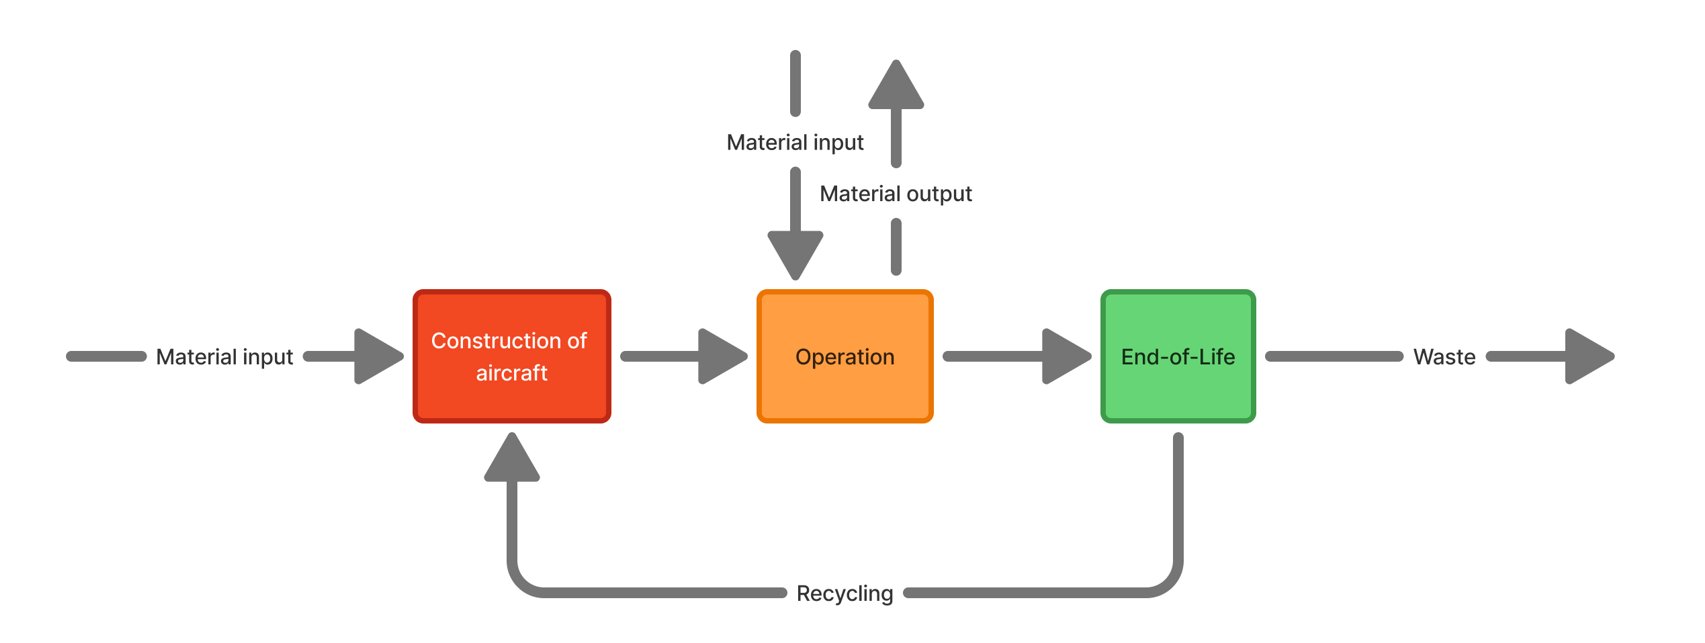
\includegraphics[width=1\linewidth]{figures/simpLCA-analysis.png}
    \caption{Simplified LCA model for the aircraft}
    \label{fig:placeholder}
\end{figure}

\end{comment}
For the LCA-analysis the software openLCA was used with the added databases: Swiss Federal Administration LCI Database (BAFU:2025) and the openLCA LCIA Methods package \footnote{\href{https://nexus.openlca.org/downloads}{openLCA Nexus} (accessed 6.05.2026)}. For the streamlined assessment the focus is on the construction of fuselage, empennage and wings. The preliminary mass together with a weight fraction can be used to estimate the weight of wings, fuselage, empennage and landing gears (the turbine is not taken into consideration since this is not part of the material selection). Different materials will lead to different weights (as the specific structural characteristics are different for each material). The complete graphs and data files for each material can be found at \footnote{\href{https://www.dropbox.com/scl/fi/d59fjeeyomrkgpxksygrg/DSE28streamlinedLCA.zip?rlkey=iy6cmqd368n8ruztcux6bf0yh&st=o02j2rds&dl=0}{Streamlined LCA}(accessed on 18.05.2026)}.   
Finally it is necessary to assess the recycle-ability of the different materials. Wood can be relatively easily be reused or can be burned as fuel.%\footnote{\href{https://www.unilinpanels.com/en/sustainability/recycling   }{UNILIN} (accessed 18.05.2026)}.  
As is often the case with metals it is possible for the recycled metal to retain most of the structural performance of the virgin material\footnote{\href{https://circulareconomy.europa.eu/platform/sites/default/files/euric_metal_recycling_factsheet.pdf}{Metal Recycling Factsheet}(accessed on 18.05.2026)}.  Recycling of glass and carbon- composites is typically very difficult and the large majority of these materials ends in landfills or are incinerated \cite{dot}.



\begin{table}[H]
\centering
\caption{Base Mechanical, Economic, and Environmental Properties of Selected Aerospace Materials (Mechanical data derived from \cite{Mouritz2012}).}
\label{tab:base-material-properties}
\renewcommand{\arraystretch}{1.2}
\begin{tabular}{|l|c|c|c|c|}
\hline
\textbf{ID}
  & \makecell{\textbf{Density} ($\rho$)\\($kg\,m^{-3}$)}
  & \makecell{\textbf{Young's}\\\textbf{Modulus} ($E$)\\(MPa)}
  & \makecell{\textbf{Specific}\\\textbf{Cost}\\(Euro\,$kg^{-1}$)} 
  & \makecell{\textbf{GWP}\\(kg $CO_2$ eq)} \\
  
\hline\hline

HUG-MAT-01 & 400  & 9000   & 0.85-1.7 & -4.17454
%\tablefootnote{\href{https://spotmaterial.com/material/spruce/sawnwood-kiln-dried/}{Spot material} (accessed 11.05.2026)}   
\\ \hline

HUG-MAT-02 & 4600 & 108100 & 21-25 & 52.51
%\tablefootnote{\href{https://spotmaterial.com/material/titanium/titanium-alloy-ti-6al-4v-grade-5-ti-6-4/}{Spot material} (accessed 11.05.2026)}    
\\ \hline

HUG-MAT-03 & 2700 & 69930  & 2.55-5.1 & 90.2384
%\tablefootnote{\href{https://spotmaterial.com/material/aluminium/7000-series-alznmgcu-7075-7475/}{Spot material} (accessed 11.05.2026)}  
\\ \hline

HUG-MAT-04 & 1850 & 49025  & 2.975-5.95 & 1019.0540
%\tablefootnote{\href{https://spotmaterial.com/material/magnesium/cast-we-alloys-we43-we54/}{Spot material} (accessed 11.05.2026)}
\\ \hline

HUG-MAT-05 & 8100 & 199260 & 8-20 & 65.02890
%\tablefootnote{\href{https://spotmaterial.com/material/alloy-steel/high-speed-tool-steel-hss-m-t/}{Spot material} (accessed 11.05.2026)}     
\\ \hline

HUG-MAT-06 & 1700 & 49980  & 25.91-32.30 & 389.27245
%\tablefootnote{\href{https://spotmaterial.com/material/carbon-fibre-cf/high-modulus-hm-ep-cf60-60-continuous-cf-hm/}{Spot material} (accessed 11.05.2026)} 
\\ \hline

HUG-MAT-07 & 2000 & 57400  & 6.5-8.7 & 67.81310
%\tablefootnote{\href{https://spotmaterial.com/material/high-modulus-glass-fibre/high-strength-s/}{Spot material} (accessed 12.05.2026)}   
\\ \hline
\end{tabular}
\end{table}



\begin{table}[H]
\centering
\caption{Derived Specific Material Indices and Economic Factors for Aerospace Structural Design \footref{url:midterm_material_selection}}
\label{tab:derived-material-properties}
\renewcommand{\arraystretch}{1.2}
\begin{tabular}{|l|c|c|c|c|c|c|}
\hline
\textbf{ID}
  & \makecell{\textbf{Specific}\\\textbf{Modulus}\\($E/\rho$)\\(GPa / $kg\,m^{-3}$)}
  & \makecell{\textbf{Column}\\\textbf{Buckling}\\($\sqrt{E}/\rho$)}
  & \makecell{\textbf{Plate}\\\textbf{Buckling}\\($\sqrt[3]{E}/\rho$)}
  & \makecell{\textbf{Specific}\\\textbf{Strength}\\($\sigma/\rho$)\\$\times10^{3}$\\(N\,m\,kg$^{-1}$)}
  & \makecell{\textbf{Specific}\\\textbf{Fracture}\\\textbf{Toughness}\\($K_{Ic}/\rho$)\\$\times10^{3}$\\(N\,m$^{1.5}$\,kg$^{-1}$)} 
  & \makecell{\textbf{Total}\\\textbf{Normalized}\\\textbf{Economic}\\\textbf{Factor}} \\
\hline\hline
HUG-MAT-01 & 22.5 & 0.24 & 0.05 & 138   & 10.0 & 0.21 \\ \hline
HUG-MAT-02 & 23.5 & 0.07 & 0.01 & 217   & 21.7 & 4.34 \\ \hline
HUG-MAT-03 & 25.9 & 0.10 & 0.02 & 174   & 10.7 & 0.68 \\ \hline
HUG-MAT-04 & 26.5 & 0.12 & 0.02 & 117   & 11.8 & 0.92 \\ \hline
HUG-MAT-05 & 24.6 & 0.06 & 0.01 & 295.6 & 4.9  & 3.80 \\ \hline
HUG-MAT-06 & 29.4 & 0.13 & 0.02 & 450   & 22.4 & 3.35 \\ \hline
HUG-MAT-07 & 28.7 & 0.12 & 0.02 & 384   & 31.0 & 0.94 \\
\hline
\end{tabular}
\end{table}

 The material cost per kg does not paint a clear picture, as it does not account for differences in mechanical properties. Therefore, the total normalized economic factor shown in \autoref{tab:derived-material-properties} is determined by dividing the material cost per kilogram by its material indices, multiplying them by their weights, and then normalizing the results.
%(e. g. 1 kg of CFRP is not equivalent in strength to 1 kg of steel). 
Lower values of the normalized economic factor point towards more cost-effective solutions. Detailed calculations regarding the economic factor of HUGO's material selection can be found in the Project HUGO Git\footref{url:midterm_material_selection}.


%To account for this, the cost per kilogram of each material was divided by its material indices, then normalized to a dimensionless value, and summed to arrive at the normalized material cost, where lower is better. The results of this can be seen in \autoref{tab:derived-material-properties}.
%The results of this analysis show that Sitka Spruce (HUG-MAT-01) is the cheapest material in terms of raw cost, whereas Titanium (HUG-MAT-02) is the most expensive. 



\begin{comment}

\begin{table}[H]
\centering
\caption{Pricing and emissions attributed to the selected aerospace materials}
\label{tab:material-economics}
\renewcommand{\arraystretch}{1.2}
\begin{tabular}{|l||c|c|}
\hline
\textbf{ID}
  & \makecell{\textbf{Specific}\\\textbf{cost}\\(euro\,$kg^{-1}$)}
  & \makecell{\textbf{Carbon}\\\textbf{Footprint}\\ ($CO_2 kg^{-1}$)} \\
\hline\hline
HUG-MAT-01\tablefootnote{\href{https://spotmaterial.com/material/spruce/sawnwood-kiln-dried/}{Spot material} (accessed 11.05.2026)}                  & 0.85-1.7 & 0.05-0.5 \\ \hline
HUG-MAT-02\tablefootnote{\href{https://spotmaterial.com/material/titanium/titanium-alloy-ti-6al-4v-grade-5-ti-6-4/}{Spot material} (accessed 11.05.2026)}              & 21-25 & 8.1-26.5 \\ \hline
HUG-MAT-03\tablefootnote{\href{https://spotmaterial.com/material/aluminium/7000-series-alznmgcu-7075-7475/}{Spot material} (accessed 11.05.2026)}          & 2.55-5.1 & 4-20\\ \hline
HUG-MAT-04\tablefootnote{\href{https://spotmaterial.com/material/magnesium/cast-we-alloys-we43-we54/}{Spot material} (accessed 11.05.2026)}               & 2.975-5.95 & 8.5-36 \\ \hline
HUG-MAT-05\tablefootnote{\href{https://spotmaterial.com/material/alloy-steel/high-speed-tool-steel-hss-m-t/}{Spot material} (accessed 11.05.2026)}    & 8-20 & 6.8 \\ \hline
HUG-MAT-06\tablefootnote{\href{https://spotmaterial.com/material/carbon-fibre-cf/high-modulus-hm-ep-cf60-60-continuous-cf-hm/}{Spot material} (accessed 11.05.2026)}    & 25,91-32.30  & 17.5-23.2 \\ \hline
HUG-MAT-07\tablefootnote{\href{https://spotmaterial.com/material/high-modulus-glass-fibre/high-strength-s/}{Spot material} (accessed 12.05.2026)}            & 6.5-8.7  & 4.8 \\
\hline
\end{tabular}
\end{table}
\end{comment}


\begin{comment}
HUG-MAT-01 has an extreme low carbon footprint which mostly stems from the extraction and  of since wood by it self extracts and binds carbon-dioxide from the atmosphere. Recycling HUG-MAT-01 is also possible though mostly due to wear and tear down-cycling is most often the most viable approach. The material can be made into small chips which can then be compressed and made into panels\footnote{\href{https://www.unilinpanels.com/en/sustainability/recycling   }{UNILIN} (accessed 18.05.2026)}. Disposing HUG-MAT-01 is also relatively simple as the material can be burned and used for energy and heating, though it is worth noting that this will be dependent on the surface coatings and treatment used on the material. Combustion will also lead to a release of the bounded carbon-dioxide. The majority of HUG-MAT-02 (Ti) can be found in relative large quantities in the earth crust but the refinement and purification is a very energy-intensive process \cite{min11121425}. The recycle-ability of HUG-MAT-02 is quite good and due to high production and refinement cost there is a clear incentive for recycling \cite{RAHIMI2025107056}. The production of both HUG-MAT-03 and HUG-MAT-04 has a large carbon footprint (see \autoref{tab:material-economics} with HUG-MAT-04 being very high due to the specific refining process used\cite{dot}. HUG-MAT-05 has a medium carbon footprint. As is often the case with metals it is possible for the recycled HUG-MAT-02,  HUG-MAT-03,  HUG-MAT-04 and HUG-MAT-05 to retain most of the structural performance of the virgin material \cite{euric_metal_recycling}. The final two materials would be HUG-MAT-06 and HUG-MAT-07. Sustainability is often presented as one of the largest issues for the broad implementation for carbon and glass-composites \cite{dot}. The production of both fibres are  extremely energy-heavy see \autoref{tab:material-economics} with especially carbon fibre having a large carbon footprint. There lies a potential sourcing the carbon from the atmosphere though this is not implemented on a industrial scale \cite{Keiner2024}. The resin used for the matrix is typically a thermoset. Recycling of these materials is typically very difficult and the large majority of glass and carbon- composites ends in landfills or are incinerated \cite{dot}
\end{comment}

\subsection{Criterion and Weight Factors for Material Selection Trade Off}
\label{sec:Mat_sel}
For the selection of material weight factors, a more holistic approach was applied, resulting in values from 0.1 to 1.0, where 1.0 warrants the highest priority. The following rationale was applied to justify the choice of specific values:

\begin{itemize}
    \item \textbf{Structural Properties (Weight 1.0):} It is in our best interest to minimize the weight of HUGO's structural components. Choosing materials with high specific modulus ($E/\rho$) and plate buckling efficiency ($\sqrt[3]{E}/\rho$) are required to withstand aeroelastic effects at Mach 0.75 while minimizing weight. Concentrated load structures (landing gear, pylons) are driven by high specific yield strength ($\sigma_y/\rho$) and fracture toughness ($K_{Ic}/\rho$) to safely absorb dynamic landing loads. Therefore, structural performance directly dictates the aerodynamic and operational feasibility of the platform. It warrants the highest trade-off weight, 1.0.
    
    \item \textbf{Durability (Weight 0.85):} HUGO is designed for a 15-year operational lifecycle with several flight days per year. The selected materials must withstand continuous high-impact cyclic loading, runway debris abrasion, and environmental degradation—including UV exposure for composites and galvanic corrosion at hybrid metallic-composite interfaces. While these issues can be solved using protective coatings and modern construction methods like using patches of fibreglass between the aluminium and carbon fibre components, the durability of the materials used is a large factor in the material selection process, warranting a weight of 0.85. 

    \item \textbf{Material Cost (Weight 0.1):} The cost of the raw materials of the structure of HUGO has a small overall impact on the financial feasibility of the project, as found in the market analysis during the previous design phase\footref{url:baseline_report}. As explained in \autoref{sec:trade-off_criteria_selection}, the overall costs are expected to be dominated by manufacturing. Therefore, this criterion was assigned the lowest weight of 0.1.
    %The costs of processing these materials and production of the parts have a far greater impact than the cost of the materials themselves. The specific costs of all the considered materials are listed in \autoref{tab:base-material-properties}.

    \item \textbf{Manufacturing Cost (Weight 0.5):} Manufacturing complexity dictates the primary financial burden of the project due to the low-volume production model. For aerodynamic surfaces, high Non-Recurring Engineering (NRE) costs associated with custom metallic tooling (e.g., stretch forming blocks) must be balanced against the high labour and autoclave operational costs of composite layups. For localized structures, direct CNC machining of metallic billets offers a highly efficient, low-NRE production route. Manufacturing methodology directly controls the economic viability of unit scaling, However, as shown in the previous design phase\footref{url:baseline_report}, there is a wide margin in the unit cost in the overall financial viability, which is why the criterion was deemed as one of medium importance, and assigned a weight of 0.5.

    \item \textbf{Design Freedom (Weight 1.0):} Project HUGO functions as a flying testbed, rather than a mass-production vehicle. Maximizing design freedom allows for the implementation of complex, aerodynamically optimized profiles and fuselage geometries, that would be impossible or prohibitively heavy if restricted to simple, developable surfaces. Because the ability to manufacture advanced aerodynamic shapes directly governs the quality of the research data the platform can generate, design freedom is classified as a primary requirement and assigned the maximum weight of 1.0.

    \item \textbf{Sustainability (Weight 0.5):} Being at the forefront of modern aviation research, HUGO shall embrace the industry's movement towards sustainable solutions. At the same time, the main design focus is the ability of HUGO to perform its mission. Therefore, this criterion was assigned a weight of 0.5.
    %The consideration of the sustainability of material has relevance for the material selection. It should always be the goal to use a material for the aircraft which is safe for the surrounding environment and where the greenhouse emissions related to its manufacture can be kept low. Due to the likely relative small size of the aircraft and the low production volume of the aircraft it has been given the weight of 0.5.
    \end{itemize}

\subsection{Trade-off table}

Based on the trade off criteria and weights selected in \autoref{sec:Mat_sel} and, the following trade off matrices were generated. Since the requirements and manufacturing methods and complexity varies significantly between the aerodynamic components (fuselage, empennage and wings), and the functional components (landing gear, pylons etc.), separate trade off matrices were required. \autoref{tab:fuselage_trade-off_matrix_material_selection} shows the trade off matrix for the aerodynamic components, and \autoref{tab:landing_gear_trade-off_matrix_material_selection} shows the trade off matrix for the functional components. 

\begin{table}[H]
\centering
\caption{Trade-Off Matrix for Fuselage, Wings and Empennage}
\renewcommand{\arraystretch}{1.4}

\begin{adjustbox}{width=\textwidth}
\begin{tabular}{|p{2.5cm}||>{\centering\arraybackslash}p{3cm}|>{\centering\arraybackslash}p{2.5cm}|>{\centering\arraybackslash}p{1.2cm}|>{\centering\arraybackslash}p{2cm}|>{\centering\arraybackslash}p{3cm}|>{\centering\arraybackslash}p{2cm}||>{\centering\arraybackslash}p{3cm}|}
\hline
\rowcolor[HTML]{4472C4}
\color{white}\textbf{Material} &\color{white}\textbf{Structural properties} &
\color{white}\textbf{Durability} &\color{white}\textbf{Materi\-al cost} &
\color{white}\textbf{Manufactur\-ing cost} &\color{white}\textbf{Design freedom} &\color{white}\textbf{\shortstack{Sustain-\\ability}} &
\color{white}\textbf{Weighted Total} \\
\hline\hline

\rowcolor[HTML]{D9E2F3}
\textbf{Weight} &
1 & 0.85 &
0.1 &
0.5 &
1 &
0.5 &
\\
\hline

HUG-MAT-01
& 4 \cellcolor[HTML]{A9D18E}
& 1 \cellcolor[HTML]{F8696B}
& 5 \cellcolor[HTML]{63BE7B}
& 3 \cellcolor[HTML]{F4E285}
& 1 \cellcolor[HTML]{F8696B}
& 5 \cellcolor[HTML]{63BE7B}
& 10.35 \\
\hline

\rowcolor[HTML]{D9E2F3}
HUG-MAT-02
& 3 \cellcolor[HTML]{F4E285}
& 5 \cellcolor[HTML]{63BE7B}
& 1 \cellcolor[HTML]{F8696B}
& 1 \cellcolor[HTML]{F8696B}
& 3 \cellcolor[HTML]{F4E285}
& 2 \cellcolor[HTML]{F4B183}
& 11.85 \\
\hline

HUG-MAT-03
& 3 \cellcolor[HTML]{F4E285}
& 4 \cellcolor[HTML]{A9D18E}
& 4 \cellcolor[HTML]{A9D18E}
& 2 \cellcolor[HTML]{F4B183}
& 3 \cellcolor[HTML]{F4E285}
& 3 \cellcolor[HTML]{F4E285}
& 12.30 \\
\hline

\rowcolor[HTML]{D9E2F3}
HUG-MAT-04
& 3 \cellcolor[HTML]{F4E285}
& 3 \cellcolor[HTML]{F4E285}
& 4 \cellcolor[HTML]{A9D18E}
& 1 \cellcolor[HTML]{F8696B}
& 3 \cellcolor[HTML]{F4E285}
& 1 \cellcolor[HTML]{F8696B}
& 9.55 \\
\hline

HUG-MAT-05
& 3 \cellcolor[HTML]{F4E285}
& 2 \cellcolor[HTML]{F4B183}
& 1 \cellcolor[HTML]{F8696B}
& 2 \cellcolor[HTML]{F4B183}
& 3 \cellcolor[HTML]{F4E285}
& 3 \cellcolor[HTML]{F4E285}
& 10.30 \\
\hline

\rowcolor[HTML]{D9E2F3}
\textbf{HUG-MAT-06}
& \textbf{5} \cellcolor[HTML]{63BE7B}
& \textbf{3} \cellcolor[HTML]{F4E285}
& \textbf{2} \cellcolor[HTML]{F4B183}
& \textbf{2} \cellcolor[HTML]{F4B183}
& \textbf{5} \cellcolor[HTML]{63BE7B}
& \textbf{1} \cellcolor[HTML]{F8696B}
& \textbf{15.10} \\
\hline

HUG-MAT-07
& 5 \cellcolor[HTML]{63BE7B}
& 3 \cellcolor[HTML]{F4E285}
& 4 \cellcolor[HTML]{A9D18E}
& 2 \cellcolor[HTML]{F4B183}
& 4 \cellcolor[HTML]{A9D18E}
& 1 \cellcolor[HTML]{F8696B}
& 14.30 \\
\hline

\end{tabular}
\end{adjustbox}
\label{tab:fuselage_trade-off_matrix_material_selection}
\end{table}

The carbon-fiber-reinforced polymer (CFRP) emerged as the clear optimal choice for the primary lifting surfaces and fuselage. Its advantage in specific modulus and plate buckling efficiency ($\sqrt[3]{E}/\rho$) is critical for a high-aspect-ratio (HAR) aircraft operating at Mach 0.75. This is what drove its score in the structural properties section. Furthermore, CFRP offers maximum design freedom, allowing for the design of complex aerodynamic profiles necessary for a flying laboratory. It also allows for the development and construction of new wing designs without large tooling costs. Utilizing CFRP ensures that weight of the fuselage and wings can be minimized, while retaining the maximum payload volume required for the 5 kg experimental payload.



\begin{table}[H]
\centering
\caption{Trade-Off Matrix for Landing gear, Pylons, and Connection Ports}
\renewcommand{\arraystretch}{1.4}

\begin{adjustbox}{width=\textwidth}
\begin{tabular}{|p{2.5cm}||>{\centering\arraybackslash}p{3cm}|>{\centering\arraybackslash}p{2.5cm}|>{\centering\arraybackslash}p{1.2cm}|>{\centering\arraybackslash}p{2cm}|>{\centering\arraybackslash}p{3cm}|>{\centering\arraybackslash}p{2cm}||>{\centering\arraybackslash}p{3cm}|}
\hline
\rowcolor[HTML]{4472C4}
\color{white}\textbf{Material} &
\color{white}\textbf{Structural properties} &
\color{white}\textbf{Durability} &
\color{white}\textbf{Materi\-al cost} &
\color{white}\textbf{Manufactur\-ing cost} &
\color{white}\textbf{Design freedom} &
\color{white}\textbf{\shortstack{Sustain-\\ability}} &
\color{white}\textbf{Weighted Total} \\
\hline\hline

\rowcolor[HTML]{D9E2F3}
\textbf{Weight} &
1 &
0.85 &
0.1 &
0.5 &
1 &
0.5 &
\\
\hline

HUG-MAT-01
& 4 \cellcolor[HTML]{A9D18E}
& 1 \cellcolor[HTML]{F8696B}
& 5 \cellcolor[HTML]{63BE7B}
& 5 \cellcolor[HTML]{63BE7B}
& 1 \cellcolor[HTML]{F8696B}
& 5 \cellcolor[HTML]{63BE7B}
& 11.35 \\
\hline

\rowcolor[HTML]{D9E2F3}
HUG-MAT-02
& 3 \cellcolor[HTML]{F4E285}
& 5 \cellcolor[HTML]{63BE7B}
& 1 \cellcolor[HTML]{F8696B}
& 3 \cellcolor[HTML]{F4E285}
& 5 \cellcolor[HTML]{63BE7B}
& 2 \cellcolor[HTML]{F4B183}
& 14.85 \\
\hline

\textbf{HUG-MAT-03}
& \textbf{3} \cellcolor[HTML]{F4E285}
& \textbf{4} \cellcolor[HTML]{A9D18E}
& \textbf{4} \cellcolor[HTML]{A9D18E}
& \textbf{4} \cellcolor[HTML]{A9D18E}
& \textbf{5} \cellcolor[HTML]{63BE7B}
& \textbf{3} \cellcolor[HTML]{F4E285}
& \textbf{15.30} \\
\hline

\rowcolor[HTML]{D9E2F3}
HUG-MAT-04
& 3 \cellcolor[HTML]{F4E285}
& 3 \cellcolor[HTML]{F4E285}
& 4 \cellcolor[HTML]{A9D18E}
& 3 \cellcolor[HTML]{F4E285}
& 5 \cellcolor[HTML]{63BE7B}
& 2 \cellcolor[HTML]{F4B183}
& 13.45 \\
\hline

HUG-MAT-05
& 3 \cellcolor[HTML]{F4E285}
& 2 \cellcolor[HTML]{F4B183}
& 1 \cellcolor[HTML]{F8696B}
& 4 \cellcolor[HTML]{A9D18E}
& 5 \cellcolor[HTML]{63BE7B}
& 3 \cellcolor[HTML]{F4E285}
& 13.30 \\
\hline

\rowcolor[HTML]{D9E2F3}
HUG-MAT-06
& 5 \cellcolor[HTML]{63BE7B}
& 3 \cellcolor[HTML]{F4E285}
& 2 \cellcolor[HTML]{F4B183}
& 1 \cellcolor[HTML]{F8696B}
& 3 \cellcolor[HTML]{F4E285}
& 1 \cellcolor[HTML]{F8696B}
& 12.60 \\
\hline

HUG-MAT-07
& 5 \cellcolor[HTML]{63BE7B}
& 3 \cellcolor[HTML]{F4E285}
& 4 \cellcolor[HTML]{A9D18E}
& 1 \cellcolor[HTML]{F8696B}
& 2 \cellcolor[HTML]{F4B183}
& 1 \cellcolor[HTML]{F8696B}
& 11.80 \\
\hline

\end{tabular}
\end{adjustbox}
\label{tab:landing_gear_trade-off_matrix_material_selection}
\end{table}
\vspace{-10}
For localized, high-stress components such as the landing gear struts, engine pylons and modular port connection points, Aluminum 7075-T76 outperformed the composite alternatives. These components require a balance of high specific fracture toughness to absorb dynamic landing impacts and high manufacturability. Aluminum 7075-T76 provides excellent specific strength ($\sigma_y/\rho$) while keeping manufacturing and material costs significantly lower than titanium or composite alternatives. The selection of high-strength aluminium heavily supports the project's modularity requirement.
%Hardpoints, pylons, and gear attachments can be rapidly CNC-machined, tapped, and modified to accommodate swappable test articles without the need for expensive composite tooling or complex inserts.
